\documentclass[a4paper,twoside]{article}

%% Language and font encodings
\usepackage[spanish]{babel}
\usepackage[utf8]{inputenc}
\usepackage[T1]{fontenc}


%% Sets page size and margins
\usepackage[a4paper,top=3cm,bottom=2cm,left=2.5cm,right=2.5cm,marginparwidth=0.5cm]{geometry}

\usepackage{amsmath}			%Paquete matemático
\usepackage{graphicx}
\usepackage[colorinlistoftodos]{todonotes}

\usepackage{hyperref}		%Paquete empleado para colocar hipervinculos
\hypersetup{
	colorlinks = true,
	linkcolor = black,
}

\usepackage{eurosym}
\usepackage{pdfpages}			%Sirve para incluir PDF en el documento
\usepackage{anysize}			%Podremos colocar imagenes de cualquier tamaño
\usepackage{subfig}				%Nos permitira colocar varias imagenes en una figura
\usepackage{float}				%Podremos crear y colocar boxes donee queramos
\usepackage[export]{adjustbox}

%Colocamos cabeceras y pies de pagina
%(CONSULTA: http://edicionesoniricas.com/maquetar-latex-encabezados-pies-pagina/)
%(CONSULTA2: https://es.sharelatex.com/learn/Headers_and_footers)
%\bfseries es análogo a \textbf{}
% \leftmark-> Adds name and number of the current top-level structure (section for article) in uppercase letters.
%\rightmark-> Adds name and number of the current next to top-level structure (subsection for article) in uppercase letters.
\usepackage{fancyhdr}		%Paquetes necesarios
\pagestyle{fancy}			%Borra los parametros por defecto
\fancyhf{}
\fancyhead[RO,LE]{\bfseries\thepage}
\fancyhead[LO,RE]{\bfseries\rightmark}
%Nos aseguramos de que en las paginas plain, no haya ni cabeceras ni lineas
\fancypagestyle{plain}
{
	\fancyhead{} % elimina cabeceras en paginas "plain"
	\renewcommand{\headrulewidth}{0pt} % así como la raya
}

%Definimos las lineas divisoras de las cabeceras y pie de pagina
\renewcommand{\headrulewidth}{1pt}	%Define el grosor de la línea de head
\renewcommand{\footrulewidth}{0pt}		%Define el grosor de la linea foot (Si no queremos linea, 0pt)
\addtolength{\headheight}{0.5pt} % espacio para la raya

%Librerias para introducir código de Matlab
%\usepackage{bigfoot} % to allow verbatim in footnote
\usepackage[numbered,framed]{matlab-prettifier}

\lstset{
	style              = Matlab-editor,
	basicstyle         = \mlttfamily,
	escapechar         = ",
	mlshowsectionrules = true,
}

% %%%%%%%%% INTRODUCIR CODIGO DE C %%%%%%%%%%%%%%%%%%%%%%
\usepackage{listings}
\usepackage{xcolor} % for setting colors

% set the default code style
%:Paquete para modificar los colores de diferentes elementos del codigo

\definecolor{mGreen}{rgb}{0,0.6,0}
\definecolor{mGray}{rgb}{0.5,0.5,0.5}
\definecolor{mPurple}{rgb}{0.58,0,0.82}
\definecolor{backgroundColour}{rgb}{0.95,0.95,0.92}

%Definimos el estilo del codigo de C
\lstdefinestyle{CStyle}{
	backgroundcolor=\color{backgroundColour},
	commentstyle=\color{mGreen},
	keywordstyle=\color{magenta},
	numberstyle=\tiny\color{mGray},
	stringstyle=\color{mPurple},
	basicstyle=\footnotesize,
	breakatwhitespace=false,
	breaklines=true,
	captionpos=b,
	keepspaces=true,
	numbers=left,
	numbersep=5pt,
	showspaces=false,
	showstringspaces=false,
	showtabs=false,
	tabsize=2,
	language=C
}
% %%%%%%%%%%%%%%%%%%%%%%%%%%%%%%%%%%%%%%%%%%%%%%%%%%

% Pie de pagina
%\fancyfoot{} % limpia el pie
\fancyfoot[C]{- \thepage -} % número de página centrado

%Nos generará texto para pruebas de maquetado
\usepackage{lipsum}

% Se varia el limite de colimnas de latex
\setcounter{MaxMatrixCols}{11}
\usepackage{lscape}
%----------------------------------------------------------------------------------------------------------------------------------
\begin{document}
\begin{titlepage}
	\centering
\Huge{\textbf{CONTROL Y PROGRAMACIÓN DE ROBOTS}} \\
\Huge{\textit{Proyecto de robots manipuladores}}\\

\vspace{1cm}
\LARGE{Grado en Ingeniería Electrónica, Mecatrónica y Robótica}\\
\rule{\textwidth}{0.1mm}
%  %%%%% Este trozo de codigo es para insertar imagenes %%%%%%%
\begin{figure}[h!]
	\centering
	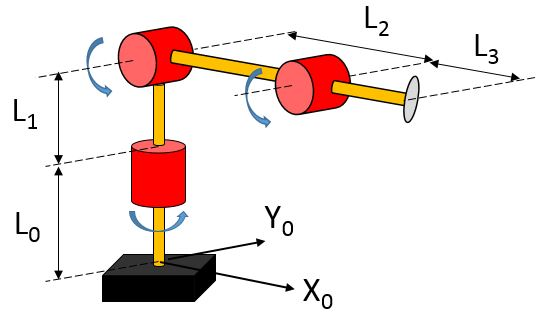
\includegraphics[width=1\textwidth]{brazo_portada}
	%\caption{textodelaleyenda}
\end{figure}
% %%%%%%%%%%%%%%%%%%%%%%%%%%%%%%%%%%%%%%%%%%%%%%%%%%%%%%%%%%%%%
\vspace{3cm}
\rule{\textwidth}{0.1mm}
\Large{\textbf{Autores:} Lozano Romero, Daniel\\
 Mérida Floriano, Javier\\
 Montes Grova, Marco Antonio}
\end{titlepage}
\tableofcontents
\newpage
% %%%%%%%%%%%   INTRODUCCION %%%%%%%%%%%%%%%%%%
\begin{abstract}
	En las páginas que siguen, se realizará un análisis cinemático y dinámico de un robot de 3 grados de libertad, cuyas articulaciones serán todas de rotación. Además de ello, debido a que únicamente se considerarán conocidas las longuitudes del robot, se deberá realizar una estimación de ciertos parámetros dinámicos del robot, como pueden ser inercias o fricciones viscosas. Finalmente, se diseñará un control cinemático y dinámico del brazo robático.\\
\end{abstract}

\section{Introducción al proyecto}
	El robot que se va a estudiar, representado por la estructura de la portada de este trabajo, posee los siguientes parámetros estructurales:
	\begin{center}
		$L_0 = 0.60 m$ \hspace{0.5 cm} $L_1 = 0.60 m$ \hspace{0.5 cm}  $L_2 = 1.00 m$\hspace{0.5 cm}  $L_3 = 0.80 m$
	\end{center}

	Además, también vienen dados los valores de factores de reducción de velocidad y constantes de par de los motores:
	\begin{center}
		$R_1 = 50; R_2 = 30; R_3 = 15$\\ \vspace{0.2 cm}
		$K_{t1} = 0.5 \frac{Nm}{A}; K_{t2} = 0.4 \frac{Nm}{A}; K_{t3} = 0.35 \frac{Nm}{A}$
	\end{center}

En primer lugar, se desarrollará un análisis cinemático del brazo robótico, tanto directo como inverso, es decir, se hallará la posición cartesiana del efector final en función de las variables articulares del brazo y viceversa.\\
Tras ello, será necesario estimar los parámetros dinámicos del brazo, ya que únicamente se conocen las longitudes del mismo. Se obtendrán diferentes parámetros en función de las condiciones supuestas para el brazo, principalmente las condiciones que se emplearan serán:
\begin{itemize}
	\item Robot con medidas ideales con reductoras.
	\item Robot con medidas ideales de accionamiento directo.
	\item Robot con medidas reales con reductoras.
	\item Robot con medidas reales de accionamiento directo.
\end{itemize}
Para el robot con medidas reales, se evaluará qué condición es mas favorable. Por ejemplo, si se obtiene un mejor modelo matemático del robot empleando únicamente encoders que conozcan las posiciones de las variables articulares y derivando numéricamente para conocer las velocidades y las aceleraciones de las mismas, o el caso en el que se empleen encoders que conozcan la posición y tacómetros que conozcan las velocidades pero derivando numéricamente para obtener las aceleraciones.\\

Una vez se hayan obtenido los modelos matemáticos de las articulaciones de los robots, se diseñará un control cinemático del mismo, el cual será un generador de trayectorias que, a partir de una posición inicial, una posición real, un número de puntos y el tiempo en que se desea que vaya de un punto a otro, generará una trayectoria de las variables articulares del robot.\\

Por último, se diseñarán una serie de controladores dinámicos para el robot, en los cuales se observe la mejoría o empeoramiento de los mismos en función del tipo de robot empleado frente a otros y del tipo de experimento realizado.\\
Además de ello, éste análisis dinámico servirá para evaluar la bondad de los modelos obtenidos para las diferentes condiciones.

% %%%%%%%%%%%%%%%%%%%%%%%%%%%%%%%%%%%%%%%%%%%%%
\newpage
\section{Análisis Cinemático del brazo}

\subsection{Modelo Cinemático Directo}

\subsubsection{Parámetros y estudio del MCD según Denavit-Hartemberg}

Uno de los modos de estudio del problema cinemático directo de un robot es el procedimiento de Denavit-Hartemberg, el cual se basa en la realización de cambios de sistema de referencia empleando las matrices de transformación homogéneas. Siguiendo una serie de pasos, se llegará a obtener los siguientes parámetros que definen la cinemática directa del robot.\\

Por tanto, los sistemas de referencia definidos se muestran a continuación:

% %%%%%%%%%%%%%%%%%

% anadir foto del analisis del brazo

% %%%%%%%%%%%%%%%%%

\begin{figure}[h!]
	
	\centering
	
	\includegraphics[width=.5\textwidth]{ejes_DH}
	
	\caption{Sistemas de referencia definidos}
	
\end{figure}



En base a esos sistemas de referencia, los parámetros de Denavit-Hartemberg obtenidos serán:

%Tabla de Denavit-Hartenberg

\begin{center}
	
	\begin{tabular}{|c||c|c|c|c|}
		
		\hline
		
		Articulación & $\theta_{i}$ & $d_{i}$ & $a_{i}$ & $\alpha_{i}$ \\
		
		\hline
		
		1 & $\theta_{1}$     				 &   L0+L1    &  			0 			 &  $\frac{\pi}{2}$  \\
		
		\hline
		
		2 & $\theta_{2}$ 				 &    0     &L2 & 0  \\
		
		\hline
		
		3 & $\theta_{3}$ &    L3    & 			 L2			 &  0\\
		
		\hline
		
	\end{tabular}
	
\end{center}



\subsubsection{Matrices de transformación homogéneas del robot}

A continuación, se mostrarán las matrices de transformación homogéneas que definen los cambios de sistema de referencia que han hecho posible relacionar el sistema de referencia base con el del efector final. La matriz de transformación homogénea que relaciona un sistema de referencia con el siguiente se define como:\\

\begin{equation}
{^{i-1}}A_{i}=Rotz(\theta_{i})*T(0,0,d_{i})*T(d_{i},0,0)*Rotx(\alpha_{i})=
\begin{pmatrix}

cos(\theta_{i}) & -sin(\alpha_{i})cos(\theta_{i})	& sin(\alpha_{i})sin(\theta_{i})  & a_{i}cos(\theta_{i})     \\

sin(\theta_{i}) &  sin(\alpha_{i})cos(\theta_{i})	& -sin(\alpha_{i})cos(\theta_{i}) & a_{i}sin(\theta_{i})     \\

0 		&  			sin(\alpha_{i})   		& 		cos(\alpha_{i})			  & d_{i}\\

0 		&					0				&				0  		  		  & 1

\end{pmatrix}
\end{equation}



Ahora que se ha definido la matriz general, se definirán las matrices de transformación homogéneas de cada cambio de sistema de referencia del robot: \\



\[ {^0}A_{1} =
\left( \begin{array}{cccc}

cos(\theta_{1}) &  0 &  sin(\theta_{1}) & 0  \\

sin(\theta_{1}) &  0 & -cos(\theta_{1}) & 0  \\

0		&  1 &		 0 			& L0+L1 \\

0		&  0 & 		 0			& 1
\end{array} \right) \]



\[ {^1}A_{2} =
\left( \begin{array}{cccc}

cos(\theta_{2}) & -sin(\theta_{2}) & 0 & L2cos(\theta_{2}) \\

sin(\theta_{2}) & cos(\theta_{2})  & 0 & L2sin(\theta_{2})  \\

0 		 	   & 			0 			& 1	& 		0 			 \\

0		 	   &			 0			& 0	& 		1
\end{array} \right) \]



\[ {^2}A_{3} =
\left( \begin{array}{cccc}

cos(\theta_{3}) &  -sin(\theta_{3}) &  0 & L3cos(\theta_{3})   \\

sin(\theta_{3}) &  cos(\theta_{3}) &  0 & L3sin(\theta_{3})   \\

0 					 &  0 &  				1 					  & 0 \\

0 					 &  0 & 				 0					  & 1
\end{array} \right) \]



\subsubsection{Ecuaciones simbólicas del MCD}

A partir de estos parámetros será posible obtener las matrices de transformación homogéneas asociadas a cada traslación y giro de sistema de referencia. Si se premultiplican las matrices desde la base hasta el punto final del brazo (efector final), la matriz de transformación obtenida será:

\begin{equation}
{^3}T_{0} =
\left( \begin{array}{cccc}

cos(\theta_{2}+\theta_{3})cos(\theta_{1})  & -sin(\theta_{2}+\theta_{3})cos(\theta_{1}) &  -sin(\theta_{1})  & cos(\theta_{1})[L3cos(\theta_{2}+\theta_{3}) + L2cos(\theta_{2})] \\

cos(\theta_{2}+\theta_{3})sin(\theta_{1})  & -sin(\theta_{2}+\theta_{3})sin(\theta_{1}) & cos(\theta_{1})  & sin(\theta_{1})[L3cos(\theta_{2}+\theta_{3}) + L2cos(\theta_{2})] \\

sin(\theta_{2}+\theta_{3})		 		  &		 cos(\theta_{2}+\theta_{3})		        & 		0 			& L0 + L1 + L3sin(\theta_{2}+\theta_{3}) + L2sin(\theta_{2})	 \\

0						  &		 	0  									&       0		    &   1
\end{array} \right)
\end{equation}

Donde se puede extraer que la matriz de orientación del efector final y la posición del mismo respecto al sistema de referencia de la base son:

\[ noa =
\left( \begin{array}{ccc}

cos(\theta_{2}+\theta_{3})cos(\theta_{1})  & -sin(\theta_{2}+\theta_{3})cos(\theta_{1}) & -sin(\theta_{1})  \\

cos(\theta_{2}+\theta_{3})sin(\theta_{1})  & -sin(\theta_{2}+\theta_{3})sin(\theta_{1}) & cos(\theta_{1})  \\

sin(\theta_{2}+\theta_{3})		 		  &		 cos(\theta_{2}+\theta_{3})		        & 		0
\end{array} \right) \]



\[ p =
\left( \begin{array}{c}

cos(\theta_{1})[L3cos(\theta_{2}+\theta_{3}) + L2cos(\theta_{2})] \\

sin(\theta_{1})[L3cos(\theta_{2}+\theta_{3}) + L2cos(\theta_{2})] \\

L0 + L1 + L3sin(\theta_{2}+\theta_{3}) + L2sin(\theta_{2})

\end{array} \right) \]



\subsection{Modelo Cinemático Inverso}



En lo que a la resolución del modelo cinemático inverso del robot respecta, se basará en obtener los valores de las variables articulares a partir de la posición del efector final. Por tanto, se partirá de las ecuaciones del vector $p$:



\begin{center}
	
	$px=cos(\theta_{1})[L3cos(\theta_{2}+\theta_{3}) + L2cos(\theta_{2})]$ \\
	
	$py=sin(\theta_{1})[L3cos(\theta_{2}+\theta_{3}) + L2cos(\theta_{2})]$ \\
	
	$pz=L0 + L1 + L3sin(\theta_{2}+\theta_{3}) + L2sin(\theta_{2})$
	
\end{center}



Para obtener las ecuaciones que definen el valor de $\theta_{1}$,$\theta_{2}$ y $\theta_{3}$, se trabajará con las funciones que definen px,py y pz. Será necesario definir los ángulos empleando la función atan2 de \textit{Matlab}, ya que de ese modo se distinguirá en qué cuadrante se encuentra la tangente.\\

Por tanto el objetivo es obtener el valor del seno y el coseno de cada ángulo.\\



Se comenzará obteniendo el valor de $\theta_{1}$. Para ello se define:\\

\begin{center}
	
	$ A = \sqrt{px^{2}+py^{2}} = L3cos(\theta_{2}+\theta_{3}) + L2cos(\theta_{2})$
	
\end{center}

de ese modo, se obtiene $\theta_{1}$ como:\\

\begin{equation}
\theta_{1}=atan2(sin(\theta_{1}),cos(\theta_{1}))=atan2(\frac{py}{A},\frac{px}{A})
\end{equation}

Para obtener el valor de $\theta_{3}$, se comenzará a partir de pz y, se definirá la siguiente variable auxiliar:\\

\begin{center}
	
	$ B=pz-L1-L0=L3sin(\theta_{2}+\theta_{3}) + L2sin(\theta_{2})$
	
\end{center}

Si se trabaja con las dos variables auxiliares creadas, A y B, y se crea la nueva variable C, se conseguirá obtener el valor del ángulo deseado:\\

\begin{center}
	
	$C= A^{2} + B^{2} = L2^{2}+ 2L2L3cos(\theta_{3}) + L3^{2} $
	
\end{center}



Cómo último paso para obtener el valor de $\theta_{3}$, se despejará el valor del coseno del mismo:\\

\begin{center}
	
	$ (cos(\theta_{3})) = \frac{C-L2^{2}-L3^{2}}{2L2L3} $
	
\end{center}

Por tanto, $\theta_{3}$ se define como:\\

\begin{equation}
\theta_{3}=\beta -atan2(sin(\theta_{3}),cos(\theta_{3}))=\beta-atan2(\pm \sqrt{1-(\frac{C-L2^{2}-L3^{2}}{2L2L3})^{2}},\frac{C-L2^{2}-L3^{2}}{2L2L3} )
\end{equation}



Por último, se hallará el valor de la variable articular $\theta_{2}$. Para ello, se partirá de la ecuación A y se desarrollará empleando la fórmula del coseno del ángulo doble. La ecuación quedará de la forma: \\

\begin{center}
	
	$A=L3cos(\theta_{2}+\theta_{3})+L2cos(\theta_{2})=L3[cos(\theta_{2})cos(\theta_{3})-sin(\theta_{2})sin(\theta_{3})]+L2cos(\theta_{2})=$\\ \vspace{0.3cm} $L3cos(\theta_{2})cos(\theta_{3})-L3sin(\theta_{2})sin(\theta_{3})+L2cos(\theta_{2})$
	
\end{center}

donde será de ayuda despejar la función A en una suma de un término por el seno de $ \theta_{2}$ y otro término por el coseno del mismo ángulo. De ese modo será posible intentar obtener dicho ángulo empleando un cambio a coordenadas polares:

\begin{center}
	
	$A=cos(\theta_{2})[L3cos(\theta_{3})+L2]-sin(\theta_{2})[L3sin(\theta_{3})]$\\
	
	\vspace{0.3cm}
	
		
		\begin{center}
			
			$\rho cos(\alpha)=L3cos(\theta_{3})+L2$ \hspace*{3cm} $\rho=\sqrt{(L3sin(\theta_{3}))^{2}+(L3cos(\theta_{3})+L2)^{2}} $\\
			
			$\rho sin(\alpha)=L3sin(\theta_{3})$ \hspace*{3.8cm} $\alpha=atan2(L3sin(\theta_{3}),L3cos(\theta_{3})+L2)$\\
			
		\end{center}
		

\end{center}

Sustituyendo en la ecuación A y empleando la fórmula del coseno del ángulo suma, se podría definir:\\

\begin{center}
	
	$A=\rho cos(\theta_{2})cos(\alpha)-\rho sin(\theta_{2})sin(\alpha)$ $\rightarrow$ $A=\rho cos(\theta_{2}+\alpha)$
	
\end{center}



Despejando el valor del coseno $\theta_{3}$ se obtendrá:

\begin{equation}
\theta_{2}=atan2(\pm \sqrt{1-(\frac{A}{\rho})^{2}},\frac{A}{\rho})-\alpha
\end{equation}

De ese modo, la solución del problema cinemático inverso está formada por siguientes ecuaciones:

\begin{center}
	
	$\theta_{1}=atan2(sin(\theta_{1}),cos(\theta_{1}))=atan2(\frac{py}{A},\frac{px}{A})$ \\
	
	$\theta_{2}=atan2(\pm \sqrt{1-(\frac{A}{\rho})^{2}},\frac{A}{\rho})-\alpha$ \\
	
	$\theta_{3}=\beta -atan2(sin(\theta_{3}),cos(\theta_{3}))=\beta-atan2(\pm \sqrt{1-(\frac{C-L2^{2}-L3^{2}}{2L2L3})^{2}},\frac{C-L2^{2}-L3^{2}}{2L2L3} )$
	
\end{center}



\subsection{Jacobiano del robot y análisis de puntos singulares}

Aunque este apartado no cabe en este proyecto, es interesante llevar a cabo el análisis de los puntos singulares del robot, los cuales se obtendrían hallando qué valores de las variables articulares del robot hacen nulo el jacobiano de velocidades, ya que esos valores de las variables articulares serán los que generen velocidades infinitas en las articulaciones del robot.\\

El jacobiano analítico de velocidades se define del siguiente modo:



\begin{equation}
J_{a} =
\begin{pmatrix}

\dfrac{\partial px}{\partial \theta_{1}} & \cdots & \dfrac{\partial px}{\partial \theta_{n}} \\

\vdots  & \ddots & \vdots  \\

\dfrac{\partial \psi}{\partial \theta_{1}} & \cdots & \dfrac{\partial \psi}{\partial \theta_{n}}
\end{pmatrix}
\end{equation}



sin embargo, debido a que no se empleará efector final y el robot posee 3 grados de libertad, no se tendrán en cuenta los ángulos de Euler que especifican la orientación del mismo, resultando la matriz jacobiana cuadrada.\\



La relación entre velocidades angulares y velocidades en el efector final se relacionan mediante el jacobiano inverso.

\begin{equation}
\begin{pmatrix}

\dot{\theta_{1}} \\

\vdots  \\

\dot{\theta_{n}}
\end{pmatrix}
= J^{-1}
\begin{pmatrix}

\dot{px} \\

\vdots  \\

\dot{\psi} \\
\end{pmatrix}
\end{equation}

Por definición, la inversa de una matriz se define como:\\

\begin{center}
	
	$ J^{-1}=\dfrac{(adj(J))^{T}}{det(J)}$
	
\end{center}

Por ello, si el determinante es nulo, el jacobiano inverso valdrá infinito y, por extensión, las velocidades en las articulaciones también lo será.\\
\newpage
\section{Control Cinemático del robot}
Una vez estudiado el análisis cinemático del modelo de brazo manipulador, y obtenidas las ecuaciones cinemáticas inversa
y directa de este, se terminará de abordar el problema cinemático, al ser capaces de desarrollar el control sobre esta; para ello,
se requiere poder generar trayectorias dentro del espacio articular, con tal de que el brazo manipulador pueda cumplir una ordenes de
movimiento conocidas.\\

Las ordenes de movimiento, en primer lugar conocidas, tendrán que especificar aquellas posiciones del espacio de trabajo,
que cumplan con la trayectoria del movimiento exigido, este primer apartado del control cinemático serán los generadores de trayectorias

% \begin{itemize}

% 	\item TIPOS DE TRAYECTORIAS. COMO LA GENERAMOS. \\
% 	Visto esto, tenemos que conocer las consignas de movimiento, mejor vistas como condiciones de contorno o exigencias,
% 	que se le piden al robot; ejemplificado en este proyecto, el movimiento del efector final entre dos puntos del espacio cartesiano
% 	del robot, dado un tiempo limite para su realización.\\

% 	\item INTERPOLADORES DE TRAYECTORIAS \rightarrow SPLINE y TRAPEZOIDAL
% 	\item IMPLEMENTACION, GRAFICAS Y CONCLUSCIONES
% \end{itemize}

\subsection{Tipos de Trayectorias Generadas}
\begin{itemize}
	\item \textsc{Generador de trayectorias lineal}\\

	Este primer generador de trayectoria trabaja con los puntos del espacio cartesiado, y con los tiempos de ejecución del movimiento; como datos
	iniciales de la orden de movimiento.
	El generador de trayectorias lineal trabaja con las ordenes de movimiento de entrada en el espacio cartesiano, y el numero de puntos intermedios
	en una trayectoria rectilinea. Con estos datos de entrada y el calculo matemático de la trayectoria se puede entregar un muestreo del número de puntos
	indicados, equidistantes en la trayectoria deseada.\\

	\begin{figure}[h!]
		\centering
		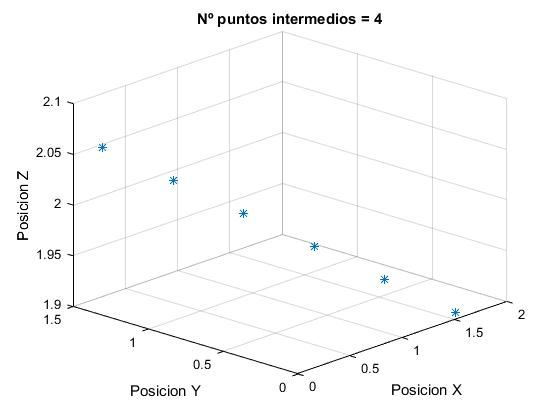
\includegraphics[width=.4\textwidth]{Lineal_4puntos} \hspace{0.25cm} 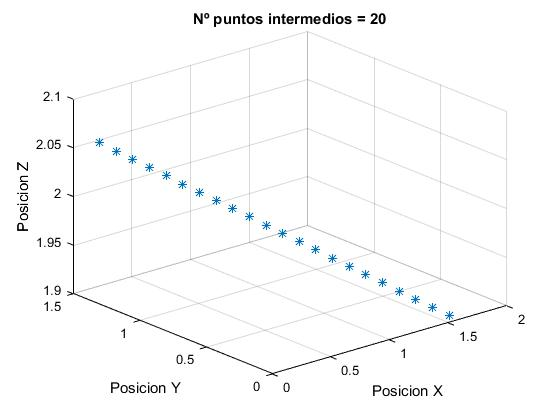
\includegraphics[width=.4\textwidth]{Lineal_20puntos}
		\caption{Generador Trayectorias lineal}
		\end{figure}

\end{itemize}

\begin{itemize}
	\item \textsc{Generador de trayectorias circular}\\

	El generador de trayectorias circulares es similar al generador de trayectorias lineal, excepto por el cálculo de la trayectoria en sí, es decir, una vez obtenidos los puntos que definen la trayectoria, se realizan los mismos cálculos para la obtención de las posiciones, velocidades y aceleraciones articulares. Se empleará también el método heurístico para definir las velocidades de paso.\\

	Para empezar, se deben introducir 3 puntos, a diferencia de los generadores lineales, que definirán la curva como punto inicial($P_1$), punto intermedio($P_2$) y punto final ($P_3$). Tras ello, se calculara el centro de la circunferencia.\\

	Primero se calcula el vector unitario perpendicular al plano definido por la circunferencia:
	\begin{center}
	$v_1=(P_2-P_1)\wedge(P_3-P_1)$\\
	$v_1=\frac{v_1}{||v_1||}$\\
	\end{center}

	Una vez obtenido dicho vector, se pasará al cálculo del centro de la circunferencia($P_0$), lo cual se realiza con un sistema de 3 ecuaciones que se resuelve de forma matricial e imponiendo que se cumplan las siguientes relaciones entre vectores (puede haber más de un sistema de ecuaciones que lleve a la resolución del problema):

	\begin{itemize}
		\item El producto escalar entre el vector $v_1$ y el vector definido por $P_0-P_1$ ha de ser nulo.\\
		\item El producto escalar entre el vector $P_0-\frac{P_2+P_1}{2}$ y el vector $P_2-P_1$ ha de ser nulo.\\
		\item El producto escalar entre el vector $P_0-\frac{P_3+P_1}{2}$ y el vector $P_3-P_1$ ha de ser nulo.\\
	\end{itemize}

	Una vez definidas las ecuaciones se ha de obtener el sistema de ecuaciones que verifique que:\\
	\begin{equation}
		P_0=A|B
	\end{equation}

	Realizando las operaciones pertinentes y despejando se pueden obtener las matrices A y B como:\\
	\begin{equation}
		A=
		\begin{bmatrix}
			v_1(1) & v_1(2) & v_1(3)\\
			P_2(1)-P_1(1) & P_2(2)-P_1(2) & P_2(3)-P_1(3)\\
			P_3(1)-P_1(1) & P_3(2)-P_1(2) & P_3(3)-P_1(3)\\
		\end{bmatrix}
	\end{equation}

\begin{equation}
		B=
		\begin{bmatrix}
			P_1(1)v_1(1)+P_1(2)v_1(2)+P_1(3)v_1(3)\\
			((P_2(1)+P_1(1))\frac{P_2(1)-P_1(1)}{2} + ((P_2(2)+P_1(2))\frac{P_2(2)-P_1(2)}{2}+((P_2(3)+P_1(3))\frac{P_2(3)-P_1(3)}{2} \\
			((P_3(1)+P_1(1))\frac{P_3(1)-P_1(1)}{2} + ((P_3(2)+P_1(2))\frac{P_3(2)-P_1(2)}{2} + ((P_3(3)+P_1(3))\frac{P_3(3)-P_1(3)}{2}\\
		\end{bmatrix}
	\end{equation}

	Una vez hallado el centro de la circunferencia, $P_0$, se debe proceder a calcular los puntos solicitados al principio del algoritmo.\\ Para ello se necesitará definir los siguientes vectores:
	\begin{equation}
		v_2=\frac{P_1-P_0}{||(P_1-P_0)||} \hspace{2cm} v_3=-\frac{v_2 \wedge v_1}{||(v_2 \wedge v_1)||}
	\end{equation}
	que serán, respectivamente, el vector unitario que va desde el centro de la circunferencia al punto $P_1$ y el vector unitario perpendicular al plano definido por $v_1$ y $v_2$ con origen en $P_1$ y sentido de la trayectoria. Con estos dos vectores, el pseudocódigo implementado para calcular los puntos que componen la trayectoria se muestra a continuación:
	\begin{center}
		$g=\frac{P_3-P_0}{||(P_3-P_0)||}$\\
		$cos_g=(v_2 \cdot g)$\\
		$sin_g=||v_2 \wedge g||$\\
		$\rho_{fin}=2\pi-atan2(sin_g,cos_g)$\\
		$\rho=linspace(0,\rho_{fin},num_{ptos})$\\
		$P=repmat(P_0,1,prod(size(\rho))+R(v_2cos(rho)+v_3sin(rho))$\\
	\end{center}

	Siendo $\rho_{fin}$ el ángulo de la posición final de la trayectoria con respecto a la posición inicial, $\rho$ el vector de N puntos de valores de ángulos desde 0 hasta el ángulo de la posición final, $R$ el radio del arco de circunferencia calculado como $R=||P_1-P_0||$, y $P$ la matriz de posiciones correspondientes a los puntos equidistantes a lo largo de la trayectoria.\\

	Una vez realizados estos pasos ya se puede pasar al cálculo de los valores de las variables articulares para las posiciones calculadas como se ha hecho anteriormente en el generador de trayectorias lineal.\\

	Los resultados obtenidos para una trayectoria específica y un valor de 100 puntos a calcular se mostrarán a continuación.
	\begin{figure}[h!]
	\centering
	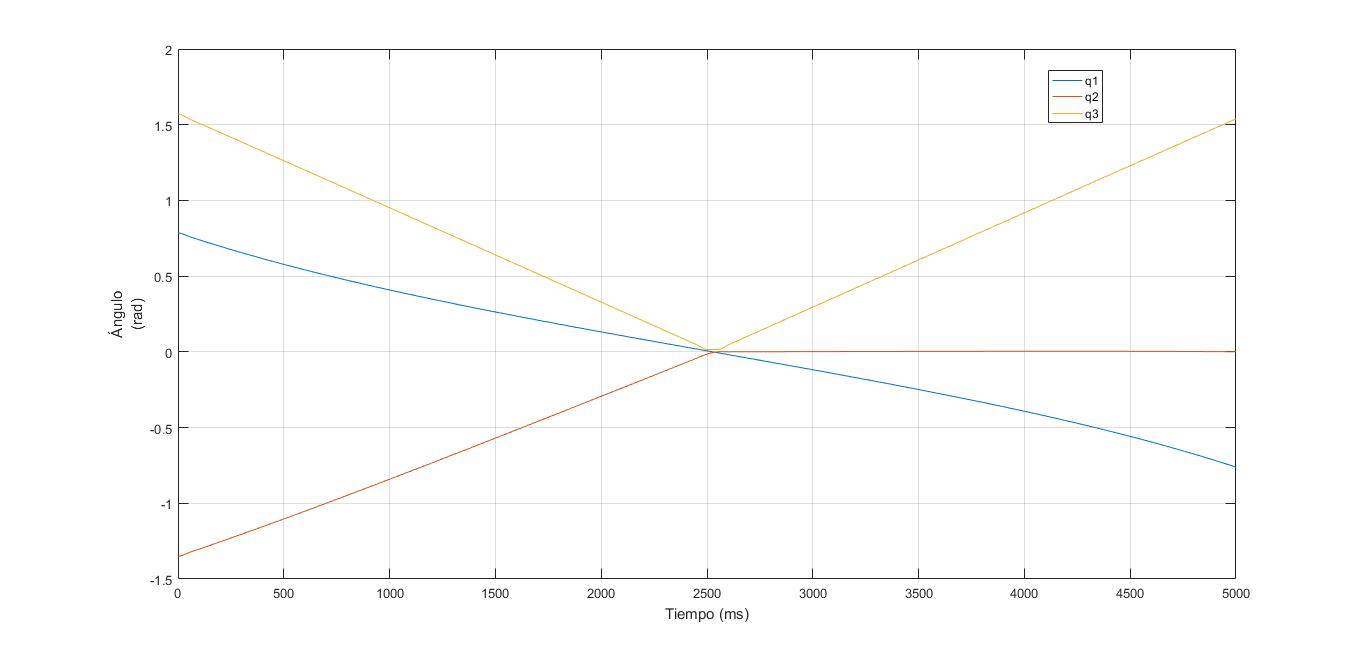
\includegraphics[width=.7\textwidth]{GDT_C_articulares}
	\caption{Valores de las variables articulares}
	\end{figure}

\newpage
Tras ello, la trayectoria ejemplo que podría seguirse en el plano XYZ será:
	\begin{figure}[h!]
	\centering
	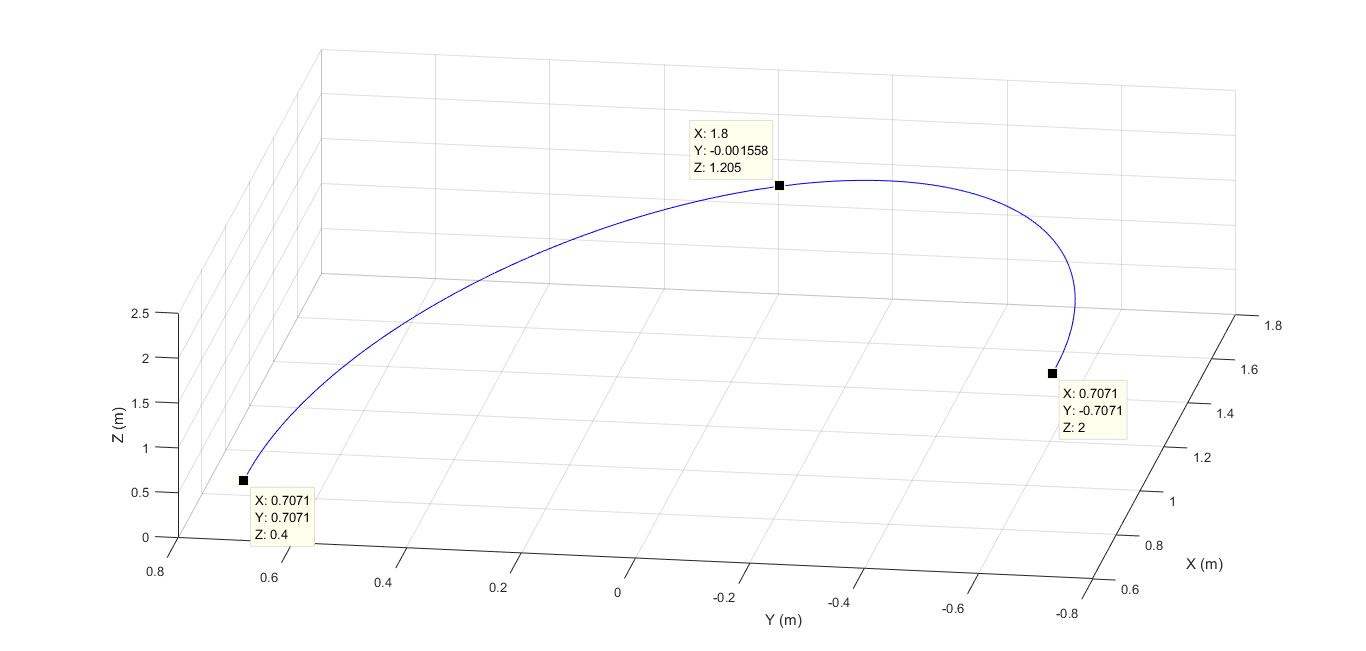
\includegraphics[width=.8\textwidth]{GDT_C_efector}
	\caption{Posición del efector final}
	\end{figure}




\end{itemize}


\subsection{Interpoladores}
Una vez obtenidos estos puntos de referencia, echaremos mano de las herramientas cedidas del análisis cinemático, ya que, se hace uso
del \textit{Modelo Cinematico Inverso}, para la obtención de los puntos de la trayectoria, representadas en el espacio de trabajo
articular del robot.\\


Una vez llegadas aquí, ya tenemos un numero de referencias articulares , que puede conllevar a un control punto a punto;
en nuestro caso, deberemos realizar un linealización de los puntos ya que debemos ser capaces de generar referencias a nuestro sistema
de forma continua. A continuación se tratara el interpolador utilizado.

	\begin{itemize}
		\item SPLINE CÚBICO.\\
		Este interpolador implementa un polinomio de 3º para dar continuidad de la trayectoria de puntos que se les entrege del
		generador pertinente, de la forma:
		\begin{center}
			\begin{equation}
				q(t)= a + b (t-t_{i}) +c (t-t_{i})^{2} + d (t-t_{i})^{3} \hspace{0.75cm};\hspace{0.75cm} t_{i}<t<t_{i+1}
			\end{equation}
			\begin{itemize}
				\item $a = q_{i} $
				\item $b = \dot{q_{i}} $
				\item $c= \frac{3}{T^{2}}(q_{i+1}-q_{i})-\frac{1}{T}(\dot{q}_{i+1}+2\dot{q}_{i})$
				\item $d= -\frac{2}{T^{3}}(q_{i+1}-q_{i})-\frac{1}{T^{2}}(\dot{q}_{i+1}+\dot{q}_{i})$
				\item $T=t_{i+1}-t_{1}$
			\end{itemize}
		\end{center}
		El trabajo matricial de esta ecuación en el espacio articular permite obtener tantos
		polinomios como tramos en la trayectoria sean exigidas por el número de puntos intermedios; pero, para ello debemos asignar valores a
		los parámetros \textit{a, b, c y d}; para estos que contengan parámetros de velocidad, se utilizará
		el método heurístico para la asignación de velocidades articulares.\\

		Le método Heurístico se basta con el análisis de la variación de las posiciones
		articulares de las muestras para asignar una velocidad de la articulación igual a cero, en el caso de que se varíe la
		dirección del movimiento; y una media entre ambas velocidades, si se aportan a la misma dirección de giro. Véase: \\

		\[
		\dot{q}_{i}= \left\{ \begin{array}{ll}
			0 & \textrm{si signo $(q_{i}-q_{i-1})$ $\neq$ signo $(q_{i+1}- q_{i})$} \\
			\frac{(q_{i+1}- q_{i})+(q_{i}-q_{i-1})}{2T} & \textrm{si signo $(q_{i}-q_{i-1})$ = signo $(q_{i+1}- q_{i})$}

		\end{array}\right.
		\]


	\end{itemize}




	\subsection{Pruebas y conclusiones}
	\begin{itemize}
		\item Objetivos: \\
		Ser capaces de que nuestro modelo de brazo manipulador ejecute ordenes de movimientos basados en trayectorias.\\

		\item Necesidad para el trabajo: \\
		Generar trayectorias de referencia en el espacio articular de nuestro modelo brazo manipulador.\\

		\item ¿Como lo hacemos? \\
		Herramientas matemáticas. que traduzcan las funcionalidades de la Orden de movimiento. \\
		Análisis Cinemático previo. Debemos poder trasladas las ordenes del espacio cartesiano, al articular del robot.
		Generar Señal de referencia. Aqui asignamos las caracteristicas de la señal de referencia; asegurar condiciones
		especificas de velocidad y aceleraciones, además de la continuidad en las consignas de referencia, apoyados en algoritmos
		de interpolación.

		\begin{figure}[h!]
			\centering
			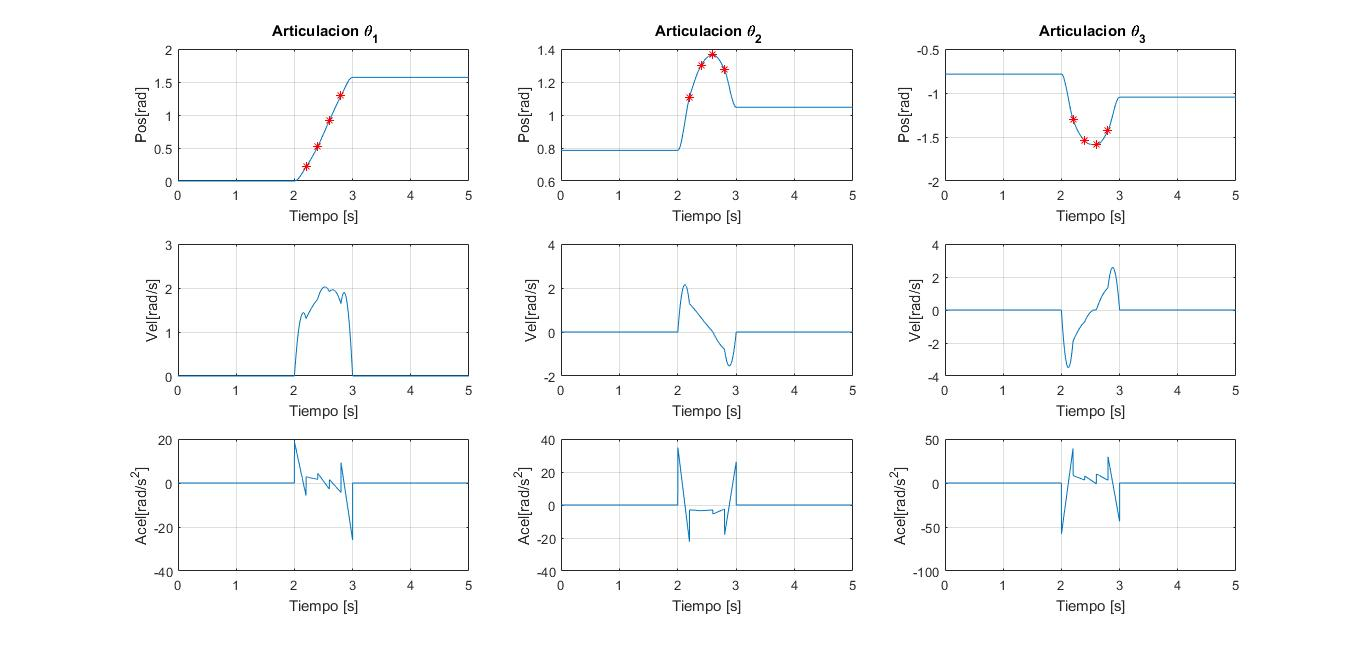
\includegraphics[width=.4\textwidth]{GeneradorTrayLineal}
			\caption{Referencia Generada Vs Referencia Entregada al Modelo}
		\end{figure}

		\newpage
		\item Resultados:
		\begin{figure}[h!]
			\centering
			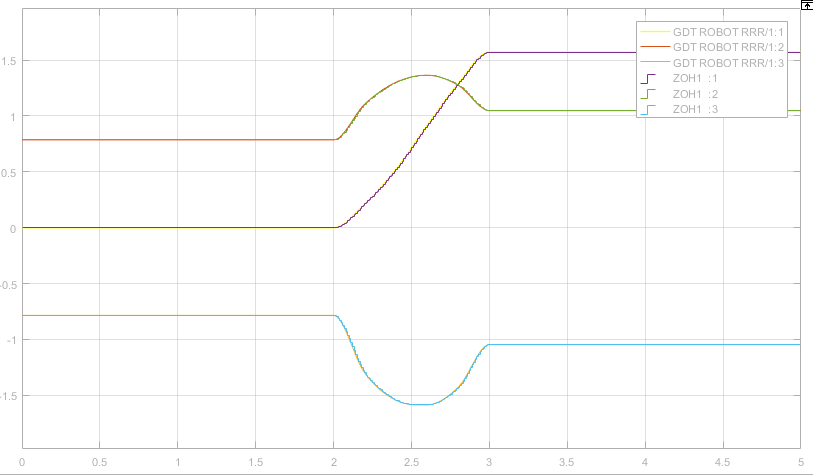
\includegraphics[width=.4\textwidth]{ZoHComparativa} \hspace{0.2cm} 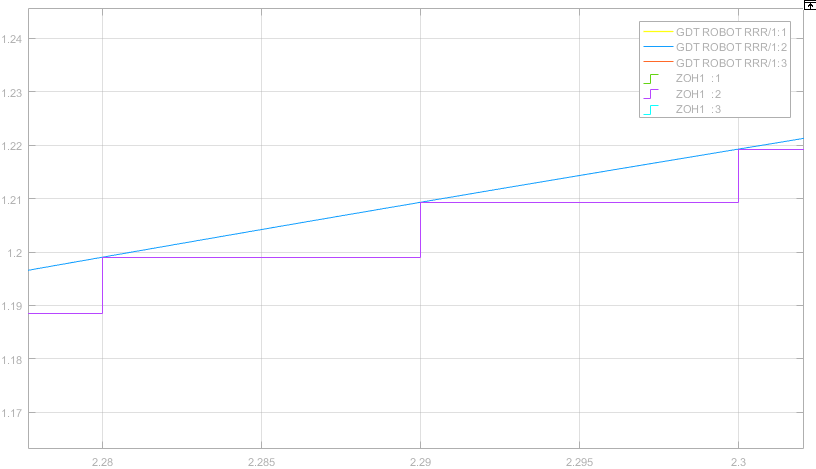
\includegraphics[width=.4\textwidth]{ZoHComparativaDetalle}
			\caption{Referencia Generada Vs Referencia Entregada al Modelo}
		\end{figure}




	\end{itemize}

\newpage
\section{Análisis Dinámico del brazo}
Una vez resuelto el problema cinemático del brazo, se debe pasar a realizar un análisis dinámico del mismo. Comenzando por un análisis que nos muestre la relación que existe entre las intensidades aplicadas a los motores de las articulaciones del robot y las posiciones, velocidades y aceleraciones de dichas articulaciones.\\
Obteniendo así, un modelo dinámico del brazo manipulador; que nos permitirá desarrollar posteriormente todas las técnicas de control propuestas, por tanto, la fiabilidad, y la exactitud del modelo obtenido, determinaran en gran medida al control que se puedan desarrollar en este proyecto.


\subsection{Modelado Dinámico e Incertidumbres}
Como se ha comenzado diciendo, se ha de ser precavido en el desarrollo de este modelo dinámico, y mas aún, de cuanto podremos fiarnos de este.\\

En primer lugar, nos basamos en el modelo estructural que permite obtener dicha relación dinámica del motor de corriente continua:\\

	\begin{equation}
	K_tRI_m=(M(q)+J_mR^2)\ddot{q}+(C(q,\dot{q})+B_mR^2)\dot{q}+G(q)+F(\dot{q})
	\end{equation}\\
	
En la ecuación anterior, se tiene; en el término de la izquierda, las matrices de constantes de par de cada motor ($K_t$) y de reductoras ($R$) e intensidades ($I_m$) aplicadas a cada motor; por otro lado, en el término de la derecha encontramos las matrices de inercia de los eslabones ($M(q)$) y de los motores ($J_m$), la matriz de términos de Coriolis ($C(q,\dot{q})$) y la de términos viscosos de los motores ($B_m$), y las matrices de términos gravitatorios ($G(q)$) y de fricciones ($F(\dot{q})$), donde esta última no se tendrá en cuenta para la estimación del modelo.\\

Aparecen también los vectores columna $q$, $\dot{q}$ y $\ddot{q}$ que corresponden, respectivamente, a los valores de posición, velocidad y aceleración de las articulaciones.\\

Teniendo la ecuación matricial, se prosigue definiendo el contenido interno de estas matrices, donde entramos a considerar las incertidumbres dinámicas del robot. Estas son, en base a la estructura tomada:
\vspace{0.3cm}

\begin{itemize}
	\item Momentos de Inercia º0:
		\begin{center}
		$ m_0$ \hspace{0.2cm} $m_1$\hspace{0.2cm} $m_2$ \hspace{0.2cm}$m_3$
		\end{center}
	\item Momentos de Inercia 1º:
		\begin{center}
		$ s_{11x}$\hspace{0.2cm} $s_{11y}$\hspace{0.2cm} $s_{11z}$\hspace{0.2cm}$ s_{22x}$\hspace{0.2cm}$ s_{22y}$\hspace{0.2cm}$ s_{22z}$\hspace{0.2cm}$ s_{33x}$\hspace{0.2cm}$ s_{33y}$\hspace{0.2cm}$ s_{33z} $
	\end{center}
	\item Momentos de Inercia 2º:
		\begin{center}
		$ I_{11xx} $\hspace{0.2cm}$I_{11yy}$\hspace{0.2cm}$ I_{11zz}$\hspace{0.2cm}$ I_{22xx}$\hspace{0.2cm}$ I_{22yy}$\hspace{0.2cm}$ I_{22zz}$\hspace{0.2cm}$ I_{33xx}$\hspace{0.2cm}$ I_{33yy}$\hspace{0.2cm}$ I_{33zz} $
	\end{center}
	\item Inercia y Fricciones de Motores:
	\begin{center}
		$Jm_1$\hspace{0.2cm}$ Jm_2 $\hspace{0.2cm}$Jm_3$\hspace{0.2cm}$ Bm_1$\hspace{0.2cm}$ Bm_2$\hspace{0.2cm}$ Bm_3$
	\end{center}
\end{itemize}

\newpage

Tras definir las incógnitas inerciales, y el conocimiento geométrico del robot, se procede a la descripcion interna de las matrices que definen nuestro modelo. Para ello, se va a realizar un método recursivo que se basa en la segunda ley de Newton denominado algoritmo de Newton-Euler, el cual obtiene los esfuerzos/pares aplicados en cada articulación.\\
 Dicho algoritmo ha sido proporcionado en clase por lo que no se explicará aquí; sí decir, que del robot sólo se conocen las longitudes de los eslabones y algunos parámetros dinámicos (reductoras y constantes de par) se realizará el cálculo con las incertidumbres dinámicas definidas como variables simbólicas que serán estimadas y sustituidas más adelante.\\

El resultado que se desea obtener con dicho algoritmo es el siguiente:\\
\begin{equation}
\tau=M(q)\ddot{q}+V(q,\dot{q})+G(q),
\end{equation}
donde el término $V(q,\dot{q})$ hace referencia al conjunto $C(q,\dot{q})\dot{q}$.\\

Como el algoritmo anterior obtiene el resultado total, se debe derivar el mismo para poder hallar las matrices aisladas. Por ello, el resultado $\tau$ se deriva respecto a $\ddot{q}$ para obtener la matriz $M(q)$. Acto seguido restar la matriz obtenida multiplicada por $\ddot{q}$ al valor de $\tau$ para eliminarlo y obtener las otras dos matrices.\\
\begin{equation}
M(q)=\dfrac{\partial{\tau}}{\partial{\ddot{q}}},
\end{equation}

El siguiente paso consiste en derivar la nueva $\tau$ respecto a la constante de gravedad $g$, puesto que aparece únicamente en los términos gravitatorios. Así, y multiplicando por $g$ a posteriori, se obtiene la matriz $G(q)$. Para hallar la matriz $V(q,\dot{q})$ basta con restar a la $\tau$ resultante de extraer la matriz de inercia la $G(q)$ anterior.\\
\begin{equation}
\tau_{new}=\tau-\dfrac{\partial{\tau}}{\partial{\ddot{q}}}\ddot{q},
\end{equation}

\begin{equation}
G(q)=\dfrac{\partial{\tau_{new}}}{\partial{g}},
\end{equation}

\begin{equation}
V(q,\dot{q})=\tau_{new}-G(q).
\end{equation}

Una de las características que hay que tener en cuenta del algoritmo de Newton-Euler es que no tiene en cuenta las viscosidades e inercias de los motores, por lo que hay que añadirlas a posteriori obteniendo las matrices $Ma(q)=M(q)+J_mR^2$ ; $Va(q,\dot{q})=V(q,\dot{q})+B_mR^2\dot{q}$ y $Ga(q)=G(q)$.\\

Una vez realizado todo esto se ha obtenido el modelo dinámico simbólico del robot, que se va a suponer correcto pues únicamente consiste en seguir unos pasos descritos en clase, pero que, si se desease, se podría comparar con un robot diseñado en Robotics Toolbox de Matlab asignando valores a los parámetros y realizando un mismo experimento para ambos modelos, tomando como referencia correcta el último de ellos.\\
\newpage
\[
Ma=
\begin{bmatrix}
Ma_{1,1} & 0 & 0\\
0 & Ma_{2,2} & Ma_{2,3}\\
0 & Ma_{3,2} & Ma_{3,3}\\
\end{bmatrix} \] 

\begin{itemize}
	\item 
	$Ma_{1,1}= I_{11yy}+0.5I_{22xx}+0.5I_{22yy}+0.5I_{33xx} +0.5I_{33yy} - 			0.5I_{22xx}cos(2q_{2})+ 0.5I_{22yy}cos(2q_2)+Jm_1R_{1}^{2} + 0.5L_{2}^{2}m_{2} +0.5L_{2}^{2}m_{3}+ 0.5L_{3}^{2}m_{3}- 0.5I_{33xx}cos(2q_{2} + 2q_{3}) +0.5I_{33yy}cos(2q_{2} + 2q_{3}) + m_{1}s{11z}^{2} + 0.5m_{2}s_{22x}^{2}+ 0.5m_{3}s_{33x}^{2}+ 0.5m_{2}s_{22x}^{2}cos(2q_{2})+ 0.5L_{3}^{2}m_{3}cos(2q_{2} + 2q_{3})+ 0.5m_{3}s{33x}^{2}cos(2q_{2}+2q_{3}) - 1.0L_{2}m_{2}s_{22x}- 1.0L_{3}m_{3}s_{33x} + 0.5L_{2}^{2}m_{2}cos(2q_{2}+ 0.5L_{2}^{2}m_{3}cos(2q_{2}+L_{2}L_{3}m_{3}cos(q_{3}) -1.0L_{2}m_{3}s_{33x}cos(q_{3})- 1.0L_{3}m_{3}s_{33x}cos(2q_{2} + 2q_{3})+L_{2}L_{3}m_{3}cos(2q_{2} + q_{3})-1.0L_{2}m_{3}s_{33x}cos(2q_{2} + q_{3})-1.0L_{2}m_{2}s_{22x}cos(2q_{2}).$ \\ 
	\vspace{0.2cm}
	
	\item $Ma_{2,2}=I_{22zz}+I_{33zz}+Jm_{2}R_{2}^{2}+L_{2}^{2}m_{2}+L_{2}^{2}m_{3}+L_{3}^{2}m_{3}+m_{2}s_{s22x}^{2}++m_{3}s_{s33x}^{2}- 2L_{2}m_{2}s_{22x}- 2L_{3}m_{3}s_{33x}+ 2L_{2}L_{3}m_{3}cos(q_{3}-2L_{2}m_{3}s_{33x}cos(q_{3})$ \\
	 \vspace{0.2cm}
	
	\item 
	$Ma_{2,3}=m_{3}L_{3}^{2}- 2L_{3}m_{3}s_{33x}+L_{2}L_{3}m_{3}cos(q_{3})+m_{3}s_{33x}^{2}-L_{2}m_{3}s_{33x}cos(q_{3})+I_{33zz}$ \\ \vspace{0.2cm}
	
	\item 
	$Ma_{3,2}=I_{33zz}+m_{3}(L_{3}-s_{33x})(L_{3}-s_{33x}+L_{2}cos(q_{3}))$ \\ 
	\vspace{0.2cm}
	
	\item 
	$Ma_{3,3}=I_{33zz}+Jm_{3}R_{3}^{2}+m_{3}(L_{3}-s_{33x})^{2}$ \\ 
	\vspace{0.2cm}

	
\end{itemize}

\[
Va=
\begin{pmatrix}
Va_{1}\\
Va_{2}\\
Va_{3}\\
\end{pmatrix} \] 
\begin{itemize}
	\item 
	$Va_{1}=Bm_{1}\dot{q_{1}}R_{1}^{2}
	-\dot{q_{1}}(I_{33yy}\dot{q_{2}} sin(2q_{2}+2q_{3}))
	-I_{33xx}\dot{q_{3}} sin(2q_{2}+2q_{3})
	-I_{33xx}\dot{q_{2}} sin(2q_{2}+2q_{3})
	+I_{33yy}\dot{q_{3}} sin(2q_{2}+2q_{3})
	-I_{22xx}\dot{q_{2}} sin(2q_{2})
	+I_{22yy}\dot{q_{2}} sin(2q_{2})
	 +m_{3}\dot{q_{2}}s_{33x}^{2}sin(2q_{2}+2q_{3})
	+m_{3}\dot{q_{3}}s_{33x}^{2}sin(2q_{2}+2q_{3})
	+L_{2}^{2}m_2 \dot{q_{2}}sin(2q_{2})
	+L_{2}^{2}m_{3}\dot{q_{2}}sin( 2q_{2})
	+m_{2}\dot{q_{2}}s_{22x}^{2}sin(2q_{2})
	+L_{3}^{2}m_{3} \dot{q_{2}}sin(2q_{2}+2q_{3})
	+L_{3}^{2}m_{3} \dot{q_{3}}sin(2q_{2}+2q_{3})
	+2L_{3}L_{2}m_{3} \dot{q_{2}}sin(2q_{2}+q_{3})
	+L_{3}L_{2}m_{3} \dot{q_{3}}sin(2q_{2}+q_{3})
	-2L_{2}m_{3}\dot{q_{2}}s_{33x}sin(2q_{2}+q_{3})
	-L_{2}m_{3}\dot{q_{3}}s_{33x}sin(2q_{2}+q_{3})
	-2L_{2}m_{2}\dot{q_{2}}s_{22x}sin(2q_{2})
	+L_{3}L_{2}m_{3} \dot{q_{3}}sin(q_{3})
	-L_{2}m_{3} \dot{q_{3}}s_{33x}sin(q_{3})
	-2L_{3}m_{3}\dot{q_{2}}s_{33x}^{2}sin(2q_{2}+2q_{3})
	-2L_{3}m_{3}\dot{q_{3}}s_{33x}^{2}sin(2q_{2}+2q_{3})
	$
	\item 
	$Va_{2}=0.5I_{33yy}\dot{q_{1}}^{2}sin(2q_{2}+2q_{3})
	-0.5I_{33xx}\dot{q_{1}}^{2}sin(2q_{2}+2q_{3})
	+Bm_{2}R_{2}^{2}\dot{q_{2}}
	-0.5I_{22xx}\dot{q_{1}}^{2}sin(2q_{2})
	+0.5I_{22yy}\dot{q_{1}}^{2}sin(2q_{2})
	+0.5L_{3}^{2}m_{3} \dot{q_{1}}^{2}sin(2q_{2}+2q_{3})
	+0.5m_{3}\dot{q_{1}}^{2}s_{33x}^{2}sin(2q_{2}+2q_{3})
	+0.5L_{2}^{2}m_{2} \dot{q_{1}}^{2}sin(2q_{2})
	+0.5L_{2}^{2}m_{3} \dot{q_{1}}^{2}sin(2q_{2})
	+0.5m_{2} \dot{q_{1}}^{2}s_{22x}^{2}sin(2q_{2})
	-L_{3}L_{2}m_{3} \dot{q_{3}}^{2}sin(q_{3})
	+L_{2}m_{3}\dot{q_{3}}^{2}s_{33x}sin(q_{3})
	-L_{3}m_{3}\dot{q_{1}}^{2}s_{33x}sin(2q_{2}+2q_{3})
	+L_{3}L_{2}m_{3} \dot{q_{1}}^{2}sin(2q_{2}+q_{3})
	-L_{2}m_{3}\dot{q_{1}}^{2}s_{33x}sin(2q_{2}+q_{3})
	-L_{2}m_{2}\dot{q_{1}}^{2}s_{22x}sin(2q_{2})
	-2L_{3}L_{2}m_{3} \dot{q_{3}}\dot{q_{2}}sin(q_{3})
	+2L_{2}m_{3} \dot{q_{2}}\dot{q_{3}}s_{33x}sin(q_{3})
	$
	
	\item 
	$Va_{3}=0.5I_{33yy}\dot{q_{1}}^{2}sin(2q_{2}+2q_{3})
	-0.5I_{33xx}\dot{q_{1}}^{2}sin(2q_{2}+2q_{3})
	+Bm_{3}R_{3}^{2}\dot{q_{3}}
	+0.5L_{3}^{2}m_{3} \dot{q_{1}}^{2}sin(2q_{2}+2q_{3})
	+0.5m_{3}\dot{q_{1}}^{2}s_{33x}^{2}sin(2q_{2}+2q_{3})
	+0.5L_{3}L_{2}m_{3} \dot{q_{1}}^{2}sin(q_{3})
	+L_{3}L_{2}m_{3} \dot{q_{2}}^{2}sin(q_{3})
	-0.5m_{3}L_{2}\dot{q_{1}}^{2}s_{33x}sin(q_{3})
	-m_{3}L_{2}\dot{q_{2}}^{2}s_{33x}sin(q_{3})
	-L_{3}m_{3}\dot{q_{1}}^{2}s_{33x}sin(2q_{2}+2q_{3})
	+0.5L_{2}L_{3}m_{3}\dot{q_{1}}^{2}sin(2q_{2}+q_{3})
	-0.5L_{2}m_{3}\dot{q_{1}}^{2}s_{33x}sin(2q_{2}+q_{3})
	$
\end{itemize}

	\[
	Ga=
	\begin{pmatrix}
	0\\
	Ga_{2}\\
	Ga_{3}\\
	\end{pmatrix} \] 
	
	\begin{itemize}
		\item 
		$Ga_{2}=g(L_{3}m_{3}cos(q_{2}+q_{3})-m_{2}s_{22x}cos(q_{2})-m_{3}s_{33x}cos(q_{2}+q_{3})+L_{2}m_{2}cos(q_{2})+L_{2}m_{3}cos(q_{2}))
		$
		
		\item 
		$Ga_{3}=g*m_{3}cos(q_{2}+q_{3})(L_{3}-s_{33x})
		$
	\end{itemize}

\newpage
%\section{Obtención de los parámetros dinámicos del robot}

Al obtener las matrices del modelo dinámico, ya seremos capaces de predecir el comportamiento de nuestro robot en la realidad;
una vez que determinemos las incertidumbres paramétricas que se especificaron al inicio del apartado anterior.
Osea se, que aunque tengamos estructuradas las matrices, no seremos capaces de determinar el comportamiento
del robot, ya que, tenemos un compendio de incertidumbres, que deberán ser determinadas numéricamente.\\


Por tanto, este apartado esclarecerá como resolver las incertidumbres paramétricas presentes, mediante
técnicas de regresión lineal y la realización de experimentos sobre el propio robot, para determinar las siguientes
incógnitas definidas en Matlab como variables simbólicas:

\begin{itemize}
	\item HABLAR UN POCO DE LA NECESIDAD DE ESTIMAR LOS PARAMETROS DE NEWTON EULER

\end{itemize}

\begin{center}
		$ I_{11} =
	\begin{bmatrix}
	I_{11xx} & I_{11xy} & I_{11xz}\\
	I_{11yx} & I_{11yy} & I_{11zz}\\
	I_{11zx} & I_{11zy} & I_{11zz}
	\end{bmatrix} $
	\vspace{0.75cm}
	$ I_{22} =
	\begin{bmatrix}
	I_{22xx} & I_{22xy} & I_{22xz}\\
	I_{22yx} & I_{22yy} & I_{22zz}\\
	I_{22zx} & I_{22zy} & I_{22zz}
	\end{bmatrix}$
	\vspace{0.75cm}
	$ I_{33} =
	\begin{bmatrix}
	I_{33xx} & I_{33xy} & I_{33xz}\\
	I_{33yx} & I_{33yy} & I_{33zz}\\
	I_{33zx} & I_{33zy} & I_{33zz}
	\end{bmatrix}$
	\vspace{0.75cm}
	$ Jm =
	\begin{bmatrix}
	Jm_{1} \\
	Jm_{2} \\
	Jm_{3}
	\end{bmatrix}$
	\vspace{0.75cm}
	$ Bm =
	\begin{bmatrix}
	Bm_{1} \\
	Bm_{2} \\
	Bm_{3}
	\end{bmatrix}$

TERMINAR DE METER MATRICES LOCO
\end{center}

	\subsection{Estimación de parámetros dinámicos}
		Primero reestructuraremos nuestro modelo dinámico en dos matrices en las que, por un lado,
		se agrupen las incertidumbres dinámicas en una matriz \textit{theta}, y por otro, el resto de nuestro modelo
		dinámico en una matriz \textit{phi} que dependerá de las variables articulares del robot.


		\begin{equation}
			\tau=M(q)\ddot{q}+V(q,\dot{q})+G(q) \hspace{1.25cm}  \rightarrow \hspace{1.25cm} \tau=\phi(x) \hspace{0.25cm} \theta
			\end{equation}



	Agrupando en \textit{theta} el conjunto de las incertidumbres obtenemos el vector de términos resultante.


	\begin{equation}
		\theta=
			\begin{pmatrix}
				I_{11xx} \\
				I_{11yy}\\
				I_{11zz}\\
				Jm_{1} \\
				Bm_{1} \\
				I_{22xx} \\
				I_{22yy}\\
				I_{22zz}\\
				Jm_{2} \\
				Bm_{2} \\
				I_{33xx} \\
				I_{33yy}\\
				I_{33zz}\\
				Jm_{3} \\
				Bm_{3} \\
				m_{1}s_{11z}^{2} \\
				m_{1}s_{11z} \\
				m_{1}\\
				m_{2}s_{22x}^{2} \\
				m_{2}s_{22x} \\
				m_{2}\\
				m_{3}s_{33x}^{2} \\
				m_{3}s_{33x} \\
				m_{3}
				\end{pmatrix}
		\end{equation}

		Si usamos esta vector \textit{theta} como base para re-ordenar nuestro modelo dinámico, vemos, en la matriz resultante \textit{phi},
		que existen columnas repletas de ceros, o relaciones lineales entre las columnas, por lo que, se deberán
		agrupar aquellos términos que no sean linealmente independientes y eliminar los términos asociados
		a las columnas de ceros, ya que significará que no tienen relevancia en nuestro modelo dinámico.\\

		Para poder agrupar los parámetros linealmente independientes, nos apoyaremos en Matlab para poder gestionar
		estas matrices de gran tamaño.\\
		Se deben dar valores aleatorios a los parámetros articulares que aparecerán en la matriz \textit{phi}, y sustituir estos
		valores dentro de la matriz; posteriormente se elegirán otros valores para las variables articulares,  y se concatenarán
		con la matriz anterior. Este proceso se repetirá hasta obtener una matriz concatenada de iguales dimensiones de ancho y largo.\\

		Obteniendo esta matriz cuadrada podremos ejecutar el comando \textit{rref()} que nos devolverá las relaciones entre las columnas de la matriz
		\textit{phi}, y que serán las mismas relaciones que dentro de las filas del vector de incertidumbres \textit{theta}.\\

		\begin{equation}
			\theta=
				\begin{pmatrix}
					  m_{1}s_{11z}^{2} + m_{2}s_{22x}^{2} + m_{3}s_{33x}^{2} + I_{11yy} + I_{22yy} + I{33yy} + R_{1}^{2}Jm_1 - m_2 - 1.64m_3 \\
					  Bm_{1}  \\
					  -m_{2}s_{22x}^{2} + I_{22xx} - I_{22yy} + m_{2} + m_{3} \\
					  m_{2}s_{22x}^{2} + I_{22zz} + R_{2}^{2}Jm_{2} - m_{2} - m_{3}  \\
					  Bm_{2} \\
					  - m_{3}s_{33x}^{2} + I_{33xx} - I_{33yy} + 0.64m_{3} \\
					  m_{3}s_{33x}^{2} + I_{33zz} - 0.64m_{3}  \\
					  Jm_{3}  \\
					  Bm_{3}  \\
					  -m_{2} -m_{3} + m_{2}s_{22x}  \\
					  m_{3}s_{33x} - 0.8m_{3}
				\end{pmatrix}
			\end{equation}



			\[
\gamma=
\begin{pmatrix}
\ddot{q_1} & R_{1}^{2}\dot{q_1} & \gamma_{1,3} & 0 & 0  & \gamma_{1,6} & 0 & 0 & 0 & \gamma_{1,10} & \gamma_{1,11} \\
0 & 0 & \gamma_{2,3} & \ddot{q_2} & R_{2}^{2}\dot{q_2} & \gamma_{2,6} & \ddot{q_2} + \ddot{q_3} & 0 & 0 & \gamma_{2,10} & \gamma_{2,11} \\
0 & 0 & 0 & 0 & 0 & \gamma_{3,6} & \ddot{q_2} + \ddot{q_3} & R_{3}^{2}\ddot{q_3} & R_{3}^{2}\ddot{q_3} & 0 & \gamma_{3,11} \\
\end{pmatrix} \] \vspace{0.3cm}

\begin{itemize}
\item $\gamma_{1,3}=\frac{\ddot{q_1}}{2} - \frac{\ddot{q_1}cos(2q_2)}{2} + \dot{q_1}\dot{q_2}sin(2q_2) $ \\ \vspace{0.2cm}
\item $\gamma_{1,6}=\frac{\ddot{q_1}}{2} - \frac{\ddot{q_1}cos(2q_2 + 2q_3)}{2} +\dot{q_1}\dot{q_2}sin(2q_2 + 2q_3) + \dot{q_1}\dot{q_3}sin(2q_2 + 2q_3) $\\ \vspace{0.2cm}
\item $\gamma_{1,10}=-L_{2}(\ddot{q_1} + \ddot{q_1}cos(2q_2) - 2\dot{q_1}\dot{q_2}sin(2q_2))$ \\ \vspace{0.2cm}
\item  $\gamma_{1,11}=2L_3\dot{q_1}\dot{q_2}sin(2q_2 + 2q_3) - L2\ddot{q_1}cos(2q_2 + q_3) - L_{3}\ddot{q_1}cos(2q_2 + 2q_3) - L2\ddot{q_1}cos(q_3) - L_{3}\ddot{q_1}$ + \\ \vspace{0.1cm}
	$+2L_{3}\dot{q_1}\dot{q_3}sin(2q_2 + 2q_3) + L_{2}\dot{q_1}\dot{q_3}sin(q_3) + 2L_{2}\dot{q_1}\dot{q_2}sin(2q_2 + q_3) + L_{2}\dot{q_1}\dot{q_3}sin(2q_2 + q_3)$ \\ \vspace{0.2cm}
\item $\gamma_{2,3}=-\frac{\dot{q_1}^{2}sin(2q_2)}{2} $\\ \vspace{0.2cm}
\item $\gamma_{2,6}=-\frac{\dot{q_1}^{2}sin(2q_2 + 2q_3)}{2} $\\ \vspace{0.2cm}
\item $\gamma_{2,10}= - L_{2}sin(2q_2)\dot{q_1}^{2} - 2L_{2}\ddot{q_2} - g*cos(q_2)$ \\ \vspace{0.2cm}
\item $\gamma_{2,11}=  L_{2}{q_3}^{2}sin(q_3) - 2L3\ddot{q_3} - g*cos(q_2 + q_3) - 2L_{3}\ddot{q_2} - L_{2}\dot{q_1}^{2}sin(2q_2 + q_3) - $\\ \vspace{0.1cm}
	$- L_{3}\dot{q_1}^{2}sin(2q_2 + 2q_3) - 2L_2\ddot{q_2}cos(q_3) - L_{2}\ddot{q_3}cos(q_3) + 2L_{2}\dot{q_2}\dot{q_3}sin(q_3) $\\ \vspace{0.2cm}
\item $\gamma_{3,6}=-\frac{\dot{q_1}^{2}sin(2q_2 + 2q_3)}{2} $\\ \vspace{0.2cm}
\item $\gamma_{3,11}=- 2L_{3}\ddot{q_2} - 2L_3\ddot{q_3} - g*cos(q_2 + q_3) - \frac{L_{2}\dot{q_1}^{2}sin(q_3)}{2} - L_2\dot{q_2}^{2}sin(q_3) - $\\ \vspace{0.1cm}
$-\frac{L_2\dot{q_1}^{2}sin(2q_2 + q_3)}{2} - L_{3}\dot{q_1}^{2}sin(2q_2 + 2q_3) - L_2\ddot{q_2}cos(q_3) $\\


Para verificar que no se ha cometido errores en este procedimiento basta con multiplicar las dos matrices obtenidas, y restarlo al modelo dinámico
que se obtuvo con el algoritmo de Newton-Euler, ya que, al ser una reorientación de parámetros, este resultado debe ser 0; por lo que
si este resultado es diferente se debe comprobar el proceso en busca de errores.
\end{itemize}

	\begin{itemize}

		\item HABLAR DE COMO SE OBTUVO GAMMA SIM Y TETHA SIM
		\item HABLAR DE LA SIMPLIFICACION A PARAMETROS LI



	\end{itemize}

	\newpage

	\subsection{Identificación y cálculos estadísticos}

	Una vez que agrupados correctamente los términos linealmente independientes de nuestra estructuradas
	\textit{phi}-\textit{theta}, se procederá a la realización de los experimentos sobre
	el robot en cuestión, y la determinación de estas incertidumbres dinámicas.\\

	Como se explicó en clases, esta identificación se basa en la regresión lineal con la minimización de los
	errores cuadráticos, para ello, necesitaremos realizar un numero de experimentos mucho mas elevado que el número
	de incertidumbres que tenemos en la matriz \textit{theta} linealmente independiente. Además, se deberá hacer
	un mínimo diseño de los experimentos a los que se va a someter el robot para la búsqueda de estos parámetros.\\

	Sobre los experimentos y la metodología que seguida. Tenemos unos parámetros están fuertemente asociados a determinados
	valores de las variables articulares; se puede ver esta dependencia al analizar el modelo dinámico de Newton-Euler.
	 Ante esto, podemos deducir a priori, que ciertos parámetros estarán mas representados ante ciertas condiciones de funcionamiento; esto será lo que determinara la
	veracidad del experimento, y de donde sacaremos las consignas para el diseño de estos.\\

	\begin{itemize}
		\item Parametros gravitarios $ \rightarrow $
		\item Parametros Inerciales $ \rightarrow $
		\item Parametros Viscosos $ \rightarrow $

	\end{itemize}







	\begin{itemize}

		\item HABLAR DE LOS EXPERIMENTOS DE LOS SENOS
		\item HABLAR DE LA OPTIMIZACION Y ESTIMACION DE LOS PARAMETROS
	\end{itemize}


	\subsection{Parametros y modelos obtenidos}
	A continuación, se mostrarán los parámetros obtenidos para cada configuración del robot, así cómo la covarianza con la que se han obtenido los mismos.\\
	Para evitar repetir siempre los parámetros, se irán definiendo componente a componente, es decir, a continuación se definirá tetha con todos los parámetros y se dirá en cada caso concreto la posición del parámetro obtenido en el vector, el valor de dicho parámetro y la covarianza del mismo. \\

	Además de ello, se obtendrán las ecuaciones dinámicas que definen el comportamiento dinámico de las articulaciones del robot. Para obtener éstas ecuaciones, será necesario multiplicar la matriz $\gamma$ que posteriormente se definirá por la matriz $\theta$ con valores numericos. \\
	Una vez se tengan las ecuaciones dinámicas del robot, al igual que se hizo cuando se aplicó el algoritmo de \textit{Newton-Euler}, se irán derivando las expresiones respecto las posiciones, velocidades y aceleraciones articulares para obtener las matrices de inercias, matriz de terminos de Coirolis y la matriz formada por los términos gravitarios.\\

	Por último, cabe destacar que los modelos con medidas reales se han obtenido a partir de la posición del modelo real cuantizada, es decir, para obtener la velocidad y la aceleración fue necesario la aplicación de filtros no causales y la aplicación de filtros que limpien los ruidos.


La matriz $\gamma$ obtenida que, multiplicada por los valores numéricos de $\theta$, resultarán las ecuaciones dinámicas del robot estudiado, se muestra a continuación:



	\subsubsection{Robot medidas ideales con reductoras}
	Los parametros estimados, es decir, la matriz tetha linealmente independiente de 11 parámetros, obtenida para desarrollar el modelo del robot con medidas ideales con reductoras en los motores será:
	\begin{center}
		\begin{tabular}{| c | c | c |}

			\hline
			Parametro estimado & Valor obtenido & Covarianza obtenida \\
			\hline
			$\theta(1) $ & 15.6322 & 0.0338 \\
			\hline
			$\theta(2) $ & 0.0012 & 0.0218 \\
			\hline
			$\theta(3) $ & 7.389 & 0.0481 \\
			\hline
			$\theta(4) $ & 55.1139 & 0.00081 \\
			\hline
			$\theta(5) $ & 0.00085 & 0.02744 \\
			\hline
			$\theta(6) $ & 2.0841 & 0.047868 \\
			\hline
			$\theta(7) $ & -2.0414 & 0.00623 \\
			\hline
			$\theta(8) $ & 0.051 & 0.00113 \\
			\hline
			$\theta(9) $ & 0.0015 & 0.033 \\
			\hline
			$\theta(10) $ & -6.665 & 0.00054 \\
			\hline
			$\theta(11) $ & -2.222 & 0.00113 \\
			\hline


		\end{tabular}
	\end{center}
Por lo tanto, tras multiplicar $\gamma$ y $\theta$ y derivar respecto a las variables articulares, se definirán las ecuaciones dinámicas del robot ideal con reductoras cómo:\\
\[
	\begin{pmatrix}
	Kt_{1}R_{1}Im_{1} \\
	Kt_{2}R_{2}Im_{2} \\
	Kt_{3}R_{3}Im_{3}
	\end{pmatrix} =
	\begin{pmatrix}
	Ma_{1,1} & 0 & 0 \\
	0 & Ma_{2,2} & Ma_{2,3}\\
	0 & Ma_{3,2} & 2.463
	\end{pmatrix}
	\begin{pmatrix}
	\ddot{q_{1}} \\
	\ddot{q_{2}}  \\
	\ddot{q_{3}}
\end{pmatrix} +
\begin{pmatrix}
	Va_{1,1}\\
	Va_{2,1} \\
  Va_{3,1}
\end{pmatrix}
\begin{pmatrix}
		\dot{q_{1}} \\
		\dot{q_{2}}  \\
		\dot{q_{3}}
\end{pmatrix} +
\begin{pmatrix}
 	0 \\
  1.81cos(q_{2} + q_{3}) + 5.44cos(q_{2}) \\
                 4.15cos(q_{2} + q_{3})
\end{pmatrix}
\]

\begin{itemize}
	\item $ Ma_{1,1}=0.0889cos(2q_{2} + q_{3}) + 0.119cos(2q_{2}) + 0.0889cos(q_{3}) + 0.0294cos(2q_{2} + 2q_{3}) + 1.15$ \\ \vspace{0.2cm}
	\item $ Ma_{2,2}=0.3703cos(q_{3}) + 5.83$ \\ \vspace{0.2cm}
	\item $ Ma_{2,3}=0.1851cos(q_{3}) + 0.126  $ \\ \vspace{0.2cm}
	\item $ Ma_{3,2}=0.4232cos(q_{3}) + 0.288  $ \\ \vspace{0.2cm}
	\item $ Va_{1,1}=0.178\dot{q_1}\dot{q_2}sin(2q_2 + q_3) + 0.0887\dot{q_1}\dot{q_3}sin(2q_2 + q_3) + 0.235\dot{q_1}\dot{q_2}sin(2q2) + 0.0887\dot{q_3}\dot{q_1}sin(q_3) + $ \\ \vspace{0.1cm}
	 $+0.059\dot{q_1}\dot{q_2}sin(2q_2 + 2q_3) + 0.059\dot{q_1}\dot{q_3}sin(2q_2 + 2q_3) - 0.12\dot{q_1} $ \\ \vspace{0.2cm}
	 \item $ Va_{2,1}=0.0638\dot{q_2} - 0.185\dot{q_3}^{2}sin(q_3) + 0.0613\dot{q_1}^{2}sin(2q_2 + 2q_3) + 0.185\dot{q_1}^{2}sin(2q_2 + q_3) + 0.248\dot{q_1}^{2}sin(2q_2) - $ \\ \vspace{0.1cm}
	 $ -0.37\dot{q_2}\dot{q_3}sin(q_3) $\\ \vspace{0.2cm}
	 \item $ Va_{3,1}= 0.0643\dot{q_3} + 0.212\dot{q_1}^{2}sin(q3) + 0.423\dot{q_2}^{2}sin(q_3) + 0.14\dot{q_1}^{2}sin(2q_2 + 2q_3) + 0.212\dot{q_1}^{2}sin(2q_2 + q_3) $
\end{itemize}

\newpage
\subsubsection{Robot medidas ideales sin reductoras}
Los parametros estimados, es decir, la matriz tetha linealmente independiente de 11 parámetros, obtenida para desarrollar el modelo del robot con medidas ideales sin reductoras en los motores será:
\begin{center}
	\begin{tabular}{| c | c | c |}

		\hline
		Parametro estimado & Valor obtenido & Covarianza obtenida \\
		\hline
		$\theta(1) $ & -9.31476 & 0.00364 \\
		\hline
		$\theta(2) $ & 0.001193 & 2.868 \\
		\hline
		$\theta(3) $ & 7.3803 & 0.00036 \\
		\hline
		$\theta(4) $ & -7.2341 & 0.00369 \\
		\hline
		$\theta(5) $ & 0.00121 & 5.890 \\
		\hline
		$\theta(6) $ & 2.078 & 0.00358 \\
		\hline
		$\theta(7) $ & -2.0335 & 0.00359 \\
		\hline
		$\theta(8) $ & 0.051 & 0.0148 \\
		\hline
		$\theta(9) $ & 0.00146 & 2.19 \\
		\hline
		$\theta(10) $ & -6.6585 & 0.003621 \\
		\hline
		$\theta(11) $ & -2.222 & 0.00356 \\
		\hline
	\end{tabular}
\end{center}
Por lo tanto, tras multiplicar $\gamma$ y $\theta$ y derivar respecto a las variables articulares, se definirán las ecuaciones dinámicas del robot ideal con reductoras cómo:\\
\[
	\begin{pmatrix}
	Kt_{1}R_{1}Im_{1} \\
	Kt_{2}R_{2}Im_{2} \\
	Kt_{3}R_{3}Im_{3}
	\end{pmatrix} =
	\begin{pmatrix}
	Ma_{1,1} & 0 & 0 \\
	0 & Ma_{2,2} & Ma_{2,3}\\
	0 & Ma_{3,2} & 4.47
	\end{pmatrix}
	\begin{pmatrix}
	\ddot{q_{1}} \\
	\ddot{q_{2}}  \\
	\ddot{q_{3}}
\end{pmatrix} +
\begin{pmatrix}
	Va_{1,1}\\
	Va_{2,1} \\
  Va_{3,1}
\end{pmatrix}
\begin{pmatrix}
		\dot{q_{1}} \\
		\dot{q_{2}}  \\
		\dot{q_{3}}
\end{pmatrix} +
\begin{pmatrix}
	0 \\
54.3cos(q_{2} + q_{3}) + 163cos(q_{2}) \\
62.1cos(q_{2} + q_{3})
\end{pmatrix}
\]

\begin{itemize}
	\item $ Ma_{1,1}=4.434cos(2q_{2} + q_{3}) + 5.937cos(2q_{2}) + 4.434cos(q_{3}) + 1.469cos(2q_{2} + 2q_{3}) + 7.693$ \\ \vspace{0.2cm}
	\item $ Ma_{2,2}=11.08cos(q_{3}) + 18.99$ \\ \vspace{0.2cm}
	\item $ Ma_{2,3}=5.542cos(q_{3}) + 3.784$ \\ \vspace{0.2cm}
	\item $ Ma_{3,2}=6.334cos(q3) + 4.325$ \\ \vspace{0.2cm}
	\item $ Va_{1,1}=-8.84\dot{q_1}\dot{q_2}sin(2q_2 + q_3) - 4.429\dot{q_1}\dot{q_3}sin(2q_2 + q_3)  -11.85\dot{q_1}\dot{q_2}sin(2q_2) - 4.429\dot{q_1}\dot{q_3}sin(q_3)-$ \\ \vspace{0.1cm}
	 $-2.924\dot{q_1}\dot{q_2}sin(2q_2 + 2q_3) - 2.924\dot{q_1}\dot{q_3}sin(2q_2 + 2q_3) 0.002387\dot{q_1} $ \\ \vspace{0.2cm}
	 \item $ Va_{2,1}=0.00304\dot{q_2} - 5.54\dot{q_3}^{2}sin(q_{3}) + 1.84\dot{q_{1}}^{2}sin(2q_{2} + 2q_{3}) + 5.54\dot{q_1}^{2}sin(2q_{2} + q_{3}) + $ \\ \vspace{0.1cm}
	 $ + 7.42\dot{q_1}^{2}sin(2q_{2}) - 11.1\dot{q_{2}}\dot{q_{3}}sin(q_{3}) ) $\\ \vspace{0.2cm}
	 \item $ Va_{3,1}=0.00418\dot{q_3} + 3.17\dot{q_1}^{2}sin(q_{3}) + 6.33\dot{q_2}^{2}sin(q_{3}) + 2.1\dot{q_1}^{2}sin(2q_{2} + 2q_{3}) + 3.17\dot{q_1}^{2}sin(2q_{2} + q_{3}) $
\end{itemize}
\newpage
\subsubsection{Robot medidas reales con reductoras}
Los parametros estimados, es decir, la matriz tetha linealmente independiente de 11 parámetros, obtenida para desarrollar el modelo del robot con medidas reales con reductoras en los motores será:
\begin{center}
	\begin{tabular}{| c | c | c |}

		\hline
		Parametro estimado & Valor obtenido & Covarianza obtenida \\
		\hline
		$\theta(1) $ & 16.995 & 4.0573 \\
		\hline
		$\theta(2) $ & 0.00122 & 0.2538 \\
		\hline
		$\theta(3) $ & 12.393 & 1.291 \\
		\hline
		$\theta(4) $ & 38.28 & 1.9472 \\
		\hline
		$\theta(5) $ & 0.00129 & 0.941 \\
		\hline
		$\theta(6) $ & 1.434 & 0.917 \\
		\hline
		$\theta(7) $ & 4.0372 & 4.545 \\
		\hline
		$\theta(8) $ & 0.0491 & 1.234 \\
		\hline
		$\theta(9) $ & 0.00151 & 1.468 \\
		\hline
		$\theta(10) $ & -6.6722 & 0.003858 \\
		\hline
		$\theta(11) $ & -2.199 & 0.008916 \\
		\hline
	\end{tabular}
\end{center}
Por lo tanto, tras multiplicar $\gamma$ y $\theta$ y derivar respecto a las variables articulares, se definirán las ecuaciones dinámicas del robot ideal con reductoras cómo:\\

\[
	\begin{pmatrix}
	Kt_{1}R_{1}Im_{1} \\
	Kt_{2}R_{2}Im_{2} \\
	Kt_{3}R_{3}Im_{3}
	\end{pmatrix} =
	\begin{pmatrix}
	Ma_{1,1} & 0 & 0 \\
	0 & Ma_{2,2} & Ma_{2,3}\\
	0 & Ma_{3,2} & 2.78
	\end{pmatrix}
	\begin{pmatrix}
	\ddot{q_{1}} \\
	\ddot{q_{2}}  \\
	\ddot{q_{3}}
\end{pmatrix} +
\begin{pmatrix}
	Va_{1,1}\\
	Va_{2,1} \\
  Va_{3,1}
\end{pmatrix}
\begin{pmatrix}
		\dot{q_{1}} \\
		\dot{q_{2}}  \\
		\dot{q_{3}}
\end{pmatrix} +
\begin{pmatrix}
	0																	\\
1.796cos(q_2 + q_3) + 5.449cos(q_2) \\
4.105cos(q_2 + q_3)
\end{pmatrix}
\]

\begin{itemize}
	\item $ Ma_{1,1}=0.088cos(2q_2 + q_3) + 0.019cos(2q_2) + 0.088cos(q_3) + 0.0417cos(2q_{2} + 2q_{3}) + 1.29$ \\ \vspace{0.2cm}
	\item $ Ma_{2,2}= 0.366cos(q_3) + 4.6$ \\ \vspace{0.2cm}
	\item $ Ma_{2,3}=0.183cos(q_3) + 0.293$ \\ \vspace{0.2cm}
	\item $ Ma_{3,2}=  0.419cos(q_3) + 0.67$ \\ \vspace{0.2cm}
	\item $ Va_{1,1}=-0.1758\dot{q_1}\dot{q_2}sin(2q_2 + q_3) - 0.08791\dot{q_1}\dot{q_3}sin(2q_2 + q_3) - 0.03796\dot{q_1}\dot{q_2}sin(2q_2) -$ \\ \vspace{0.1cm}
	 $ - 0.08791\dot{q_1}\dot{q_3}sin(q_3) - 0.08325\dot{q_1}\dot{q_2}sin(2q_2 + 2q_3) - 0.08325\dot{q_1}\dot{q_3}sin(2q_2 + 2q_3) + 0.1223\dot{q_1)}$ \\ \vspace{0.2cm}
	 \item $ Va_{2,1}=0.0969\dot{q_2} - 0.183\dot{q_3}^{2}sin(q_3) + 0.0868\dot{q_1}^{2}sin(2q_{2} + 2q_{3}) + 0.183\dot{q_1}^{2}sin(2q_2 + q_3) + $ \\ \vspace{0.1cm}
	 $ + 0.0396\dot{q_1}^{2}sin(2q_{2}) - 0.366\dot{q_2}\dot{q_3}sin(q_3) $\\ \vspace{0.2cm}
	 \item $ Va_{3,1}=0.0648\dot{q_3} + 0.209\dot{q_1}^{2}sin(q_3) + 0.419\dot{q_2}^{2}sin(q_3) + 0.199\dot{q_1}^{2}sin(2q_2 + 2q_3) + 0.209\dot{q_1}^{2}sin(2q_2 + q_3) $
\end{itemize}

\newpage
\subsubsection{Robot medidas reales sin reductoras}
Los parametros estimados, es decir, la matriz tetha linealmente independiente de 11 parámetros, obtenida para desarrollar el modelo del robot con medidas reales sin reductoras en los motores será:
\begin{center}
	\begin{tabular}{| c | c | c |}

		\hline
		Parametro estimado & Valor obtenido & Covarianza obtenida \\
		\hline
		$\theta(1) $ & - & - \\
		\hline
		$\theta(2) $ & - & - \\
		\hline
		$\theta(3) $ & - & - \\
		\hline
		$\theta(4) $ & - & - \\
		\hline
		$\theta(5) $ & - & - \\
		\hline
		$\theta(6) $ & - & - \\
		\hline
		$\theta(7) $ & - & - \\
		\hline
		$\theta(8) $ & - & - \\
		\hline
		$\theta(9) $ & - & - \\
		\hline
		$\theta(10) $ & - & - \\
		\hline
		$\theta(11) $ & - & - \\
		\hline
	\end{tabular}
\end{center}
Por lo tanto, tras multiplicar $\gamma$ y $\theta$ y derivar respecto a las variables articulares, se definirán las ecuaciones dinámicas del robot ideal con reductoras cómo:\\
\[
	\begin{pmatrix}
	Kt_{1}R_{1}Im_{1} \\
	Kt_{2}R_{2}Im_{2} \\
	Kt_{3}R_{3}Im_{3}
	\end{pmatrix} =
	\begin{pmatrix}
	Ma_{1,1} & 0 & 0 \\
	0 & Ma_{2,2} & Ma_{2,3}\\
	0 & Ma_{3,2} & -
	\end{pmatrix}
	\begin{pmatrix}
	\ddot{q_{1}} \\
	\ddot{q_{2}}  \\
	\ddot{q_{3}}
\end{pmatrix} +
\begin{pmatrix}
	Va_{1,1}\\
	Va_{2,1} \\
  Va_{3,1}
\end{pmatrix}
\begin{pmatrix}
		\dot{q_{1}} \\
		\dot{q_{2}}  \\
		\dot{q_{3}}
\end{pmatrix} +
\begin{pmatrix}
-	\\
- \\
-
\end{pmatrix}
\]
{}
\begin{itemize}
	\item $ Ma_{1,1}=$ \\ \vspace{0.2cm}
	\item $ Ma_{2,2}= $ \\ \vspace{0.2cm}
	\item $ Ma_{2,3}=$ \\ \vspace{0.2cm}
	\item $ Ma_{3,2}=  $ \\ \vspace{0.2cm}
	\item $ Va_{1,1}= $ \\ \vspace{0.2cm}
	 \item $ Va_{2,1}= $ \\ \vspace{0.2cm}
	 \item $ Va_{3,1}= $
\end{itemize}


\newpage
\subsection{Verificación de los modelos obtenidos}
Tras obtener éstos modelos, se hará una simple prueba antes de comenzar a controlar el robot para poder analizar la bondad del modelo obtenido.\\
Se ha optado por, para comprobar dicha bondad, introducirle al robot dado por el profesor, es decir, el robot real valores de intensidades unitarios y lo
mismo al modelo, de ese modo se podrá observar y comparar la respuesta del robot real y el modelo obtenido.\\

Cabe destacar que, debido a que no se controlará el robot durante más de 5 segudos aproximadamente, durante ese tiempo es dónde interesa observar la bondad del modelo.
\subsubsection{Robot medidas ideales con reductoras}
En primer lugar, se mostrará cómo responden las variables articulares del modelo obtenido frente a las del robot real. La gráfica que se muestra es la obtenida empleando las medidas ideales de éstas variables articulares tanto del robot real cómo del modelo:

\begin{figure}[h!]
	\centering
	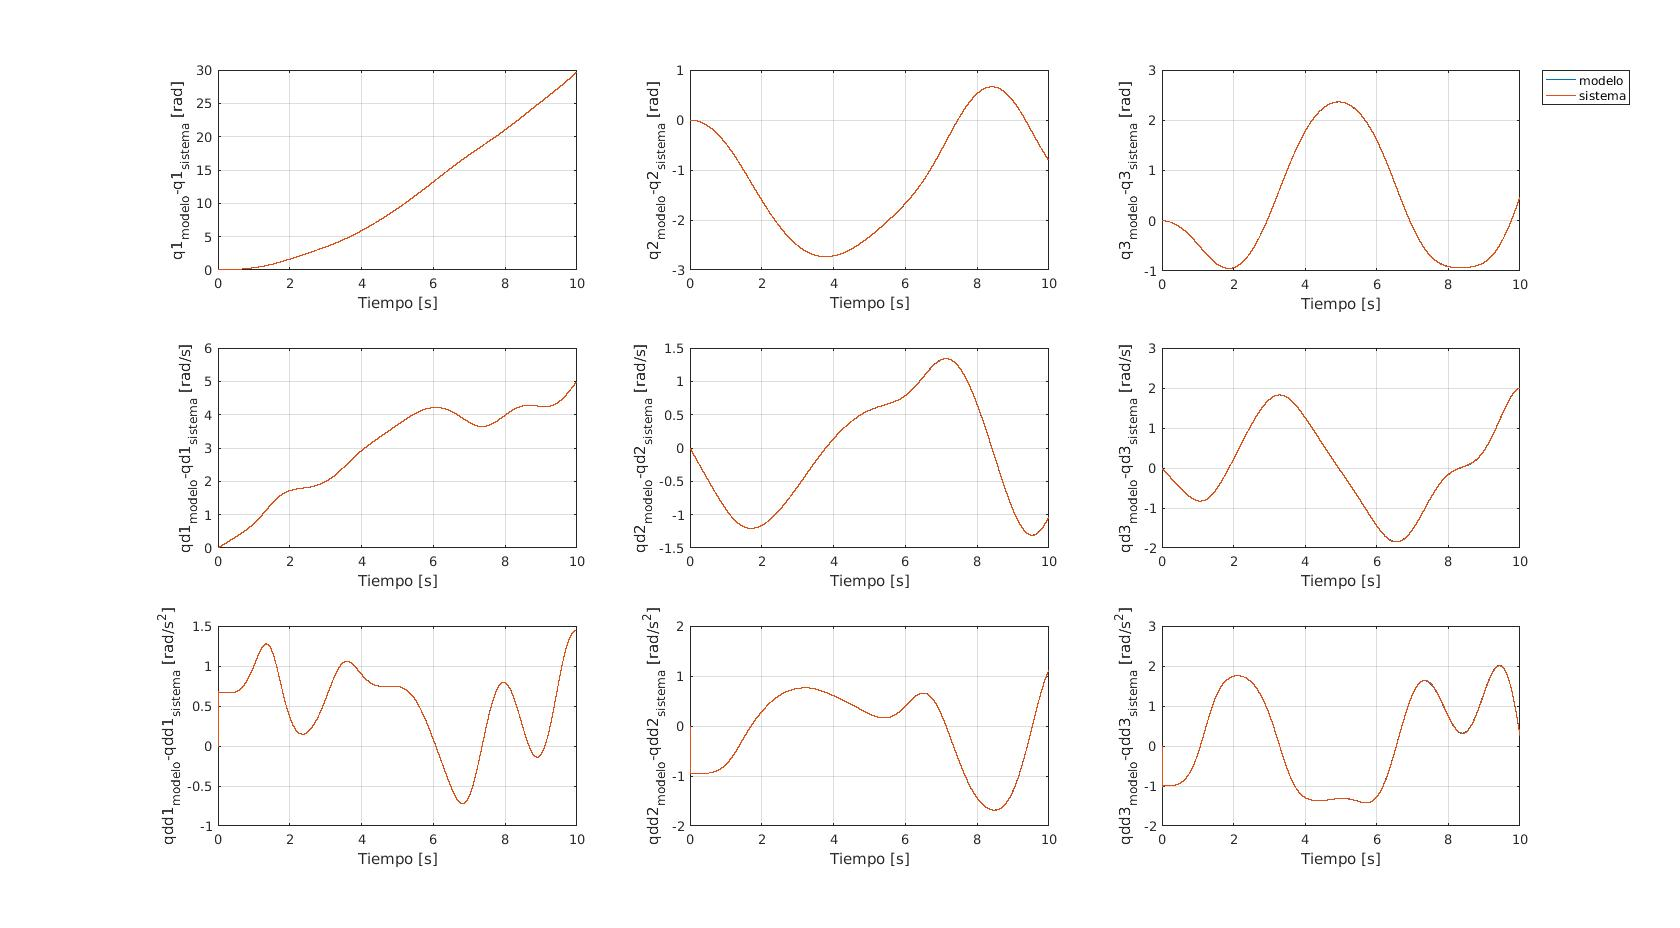
\includegraphics[width=1\textwidth]{EstimacParam_SisMod_In1_IdealCR}
	\caption{Comparativa Variables articulares del modelo obtenido con medidas ideales y reductoras}
\end{figure}

Cómo se puede observar, la magnitud del error será muy baja, por tanto, eso conllevará que se han estimado los parámetros dinámicos del robot con un bajo error entre los parámetros reales.\\
\newpage
A continuación, se mostrará la gráfica del error en las variables articulares:

\begin{figure}[h!]
	\centering
	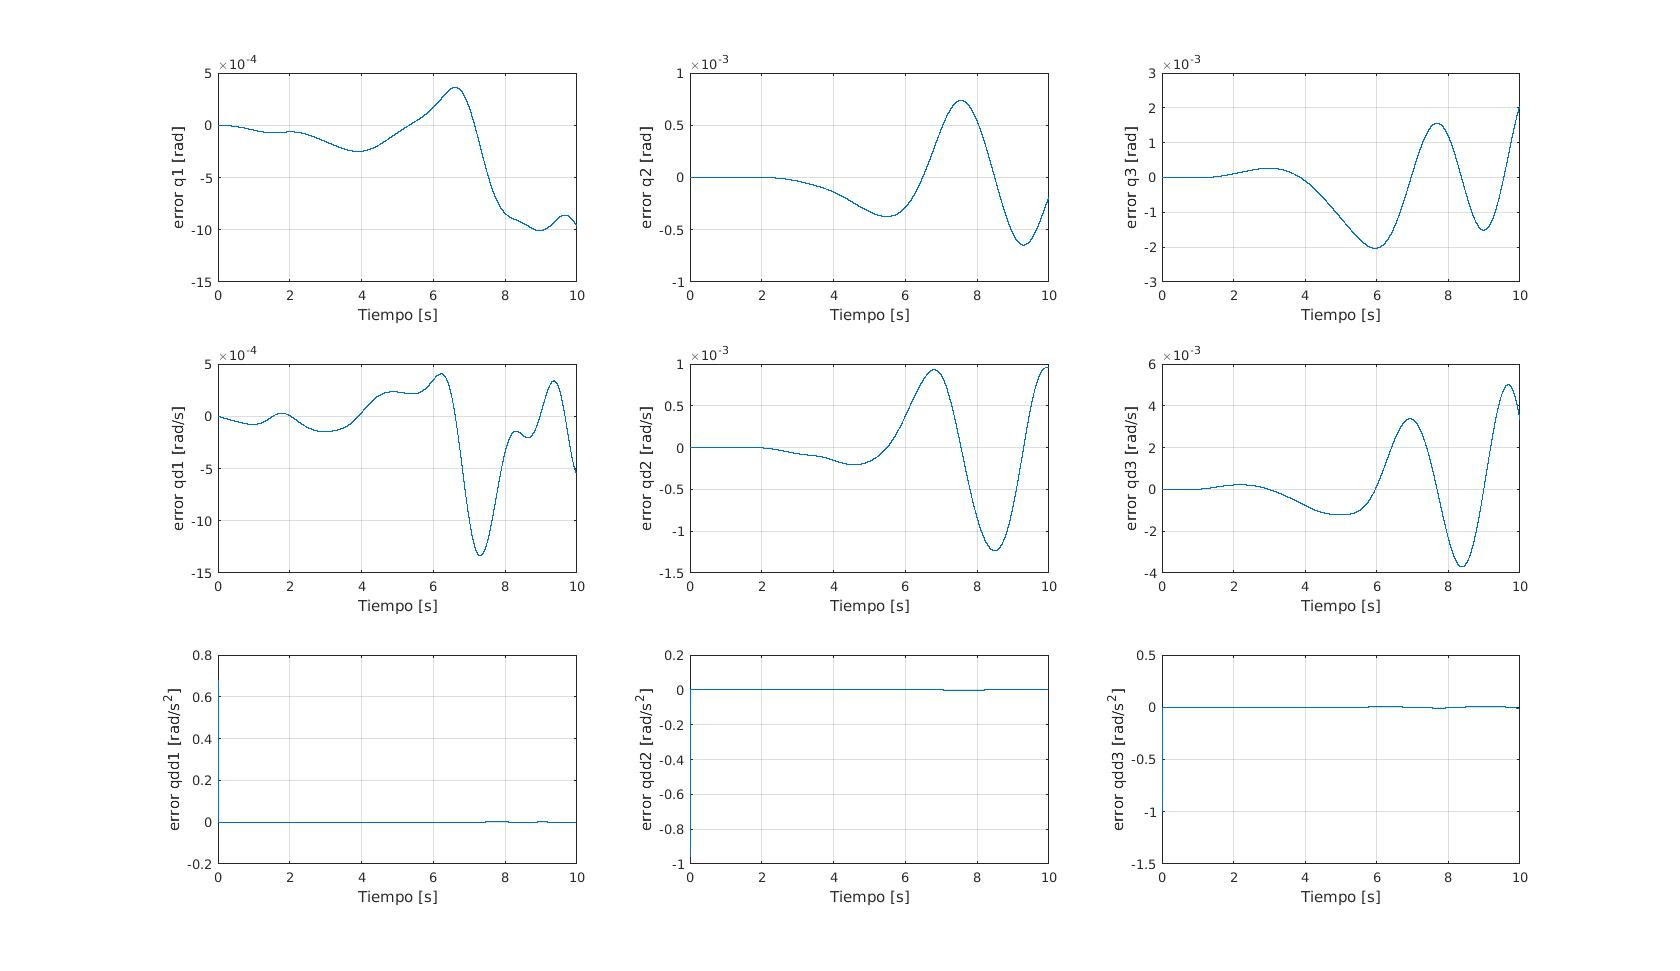
\includegraphics[width=1\textwidth]{EstimacParam_SisModError_In1_IdealCR}
	\caption{Error del modelo obtenido con medidas ideales y reductoras}
\end{figure}

\subsubsection{Robot medidas ideales sin reductoras}
En éste caso, se realizará la misma comparativa que en el caso anterior, con la salvedad es que en el modelo obtenido ahora, se suponen que no se tienen reductoras.\\
Cabe destacar que nos interesa el modelo del robot a bjos tiempos, es decir, los primeros 5 segundos de la simulación, pues no se va a querer controlar el robot en trayectorias que duren más tiempo. Se ha graficado más tiempo para que se observe que, cuando empieza a pasar más del tiempo que se desea controlar, los errores comienzan a incrementarse.\\
A continuación, se mostrará la gráfica resultando al excitar el modelo del sistema y el robot real con intensidades constantes y unitarias.

\newpage
\begin{figure}[h!]
	\centering
	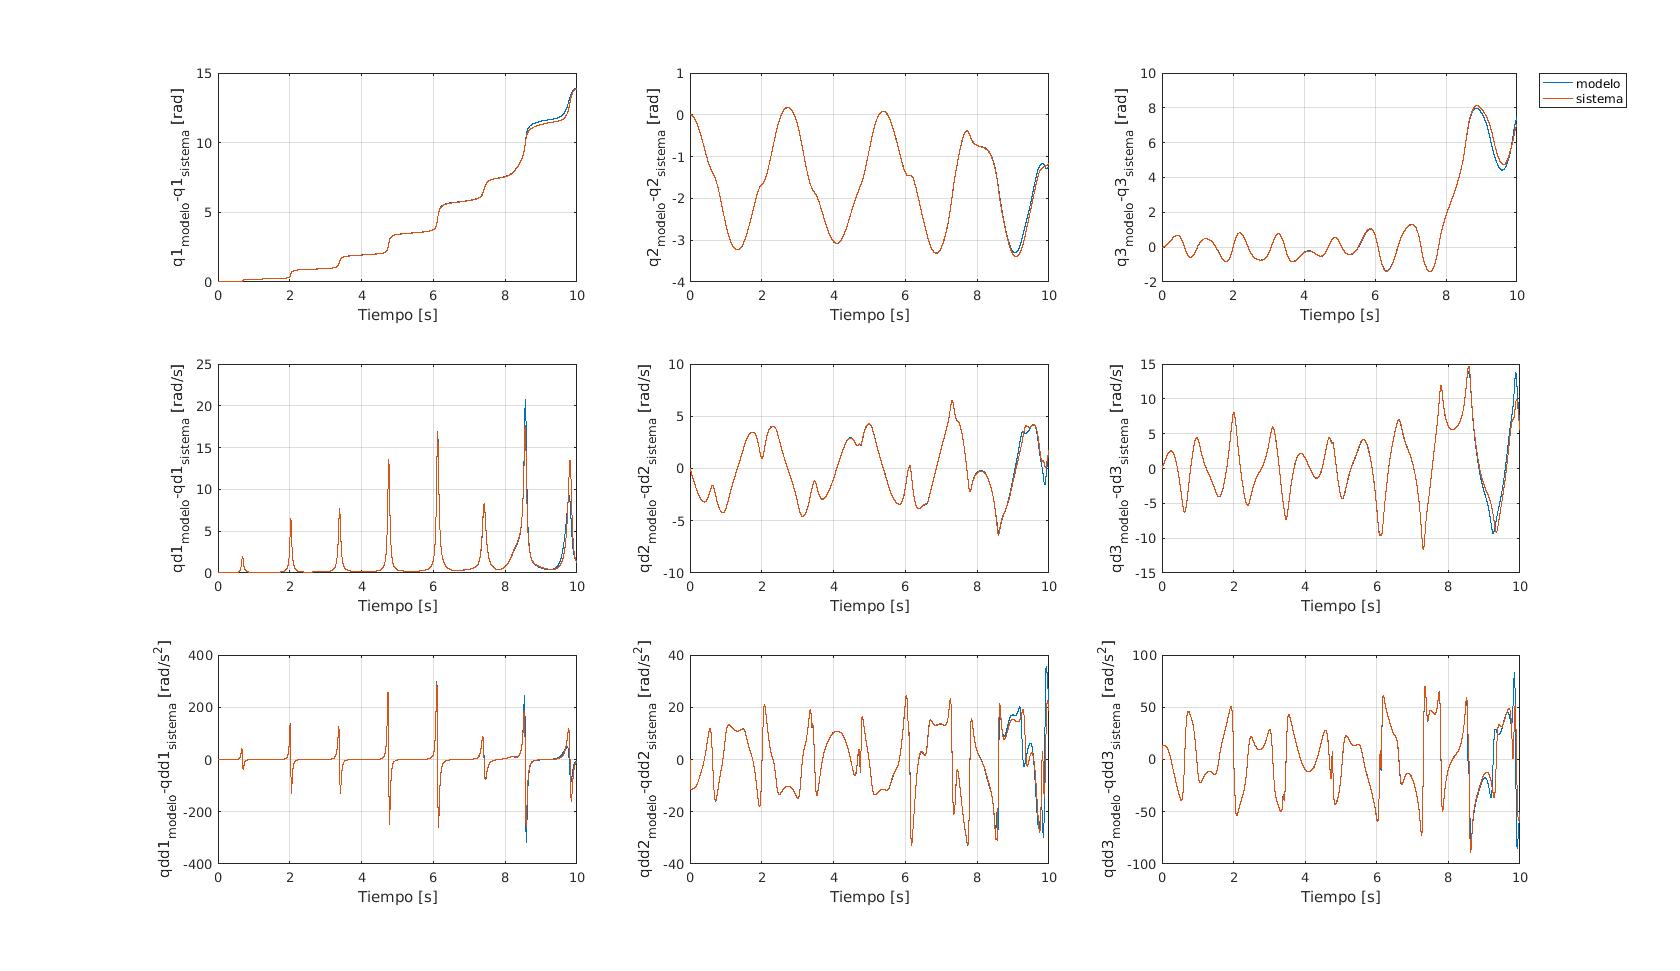
\includegraphics[width=1\textwidth]{EstimacParam_SisMod_In1_IdealSR}
	\caption{Comparativa Variables articulares del modelo obtenido con medidas ideales y sin reductoras}
\end{figure}

Cómo se puede observar, al igual que antes, cuándo se emplean medidas ideales para estimar los parámetros dinámicos del robot y obtener un modelo del mismo, se obtendrán buenos modelos, debido a que cómo se indico antes, las medidas son ideales. \\
Por tanto, a continuación se mostrará la gráfica de los errores de las variables articulares:

\begin{figure}[h!]
	\centering
	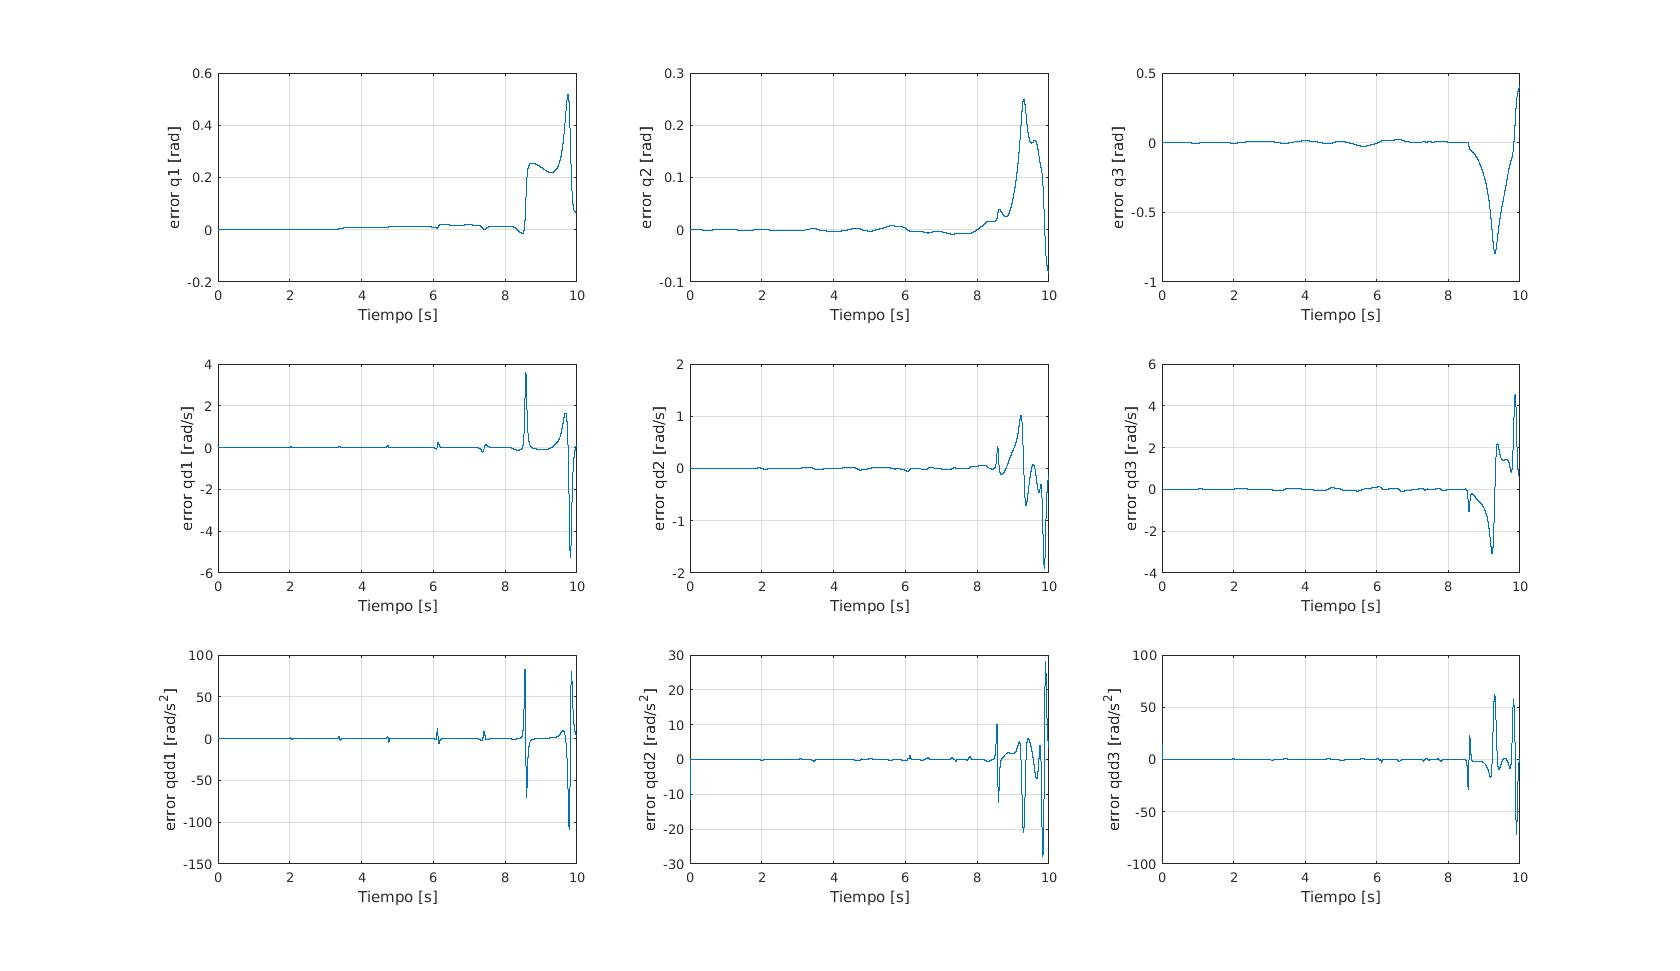
\includegraphics[width=1\textwidth]{EstimacParam_SisModError_In1_IdealSR}
	\caption{Error del modelo obtenido con medidas ideales y sin reductoras}
\end{figure}

\subsubsection{Robot medidas reales con reductoras}
Aunque se haya obtenido el modelo con medidas reales suponiendo que no se tienen tacómetros y que, por tanto, no se puede conocer la velocidad articular del robot, para realizar análisis de control y para análizar el modelo obtenido sí se conocerá la velocidad articular, es decir, se supondrá que se tienen tacómetros. De ese modo se evitará la necesidad de implementar un filtro no causal. \\
Los filtros no causales se caracterizan por el hecho de se emplean valores futuros de la señal, algo que sólo se podrá hacer de manera computacional una vez se hayan tomado todos los datos.\\

Por tanto, se compararán las medidas reales de velocidad y posición del robot con las medidas ideales del modelo obtenido. La grafica comparativa se muestra a continuación:

\begin{figure}[h!]
	\centering
	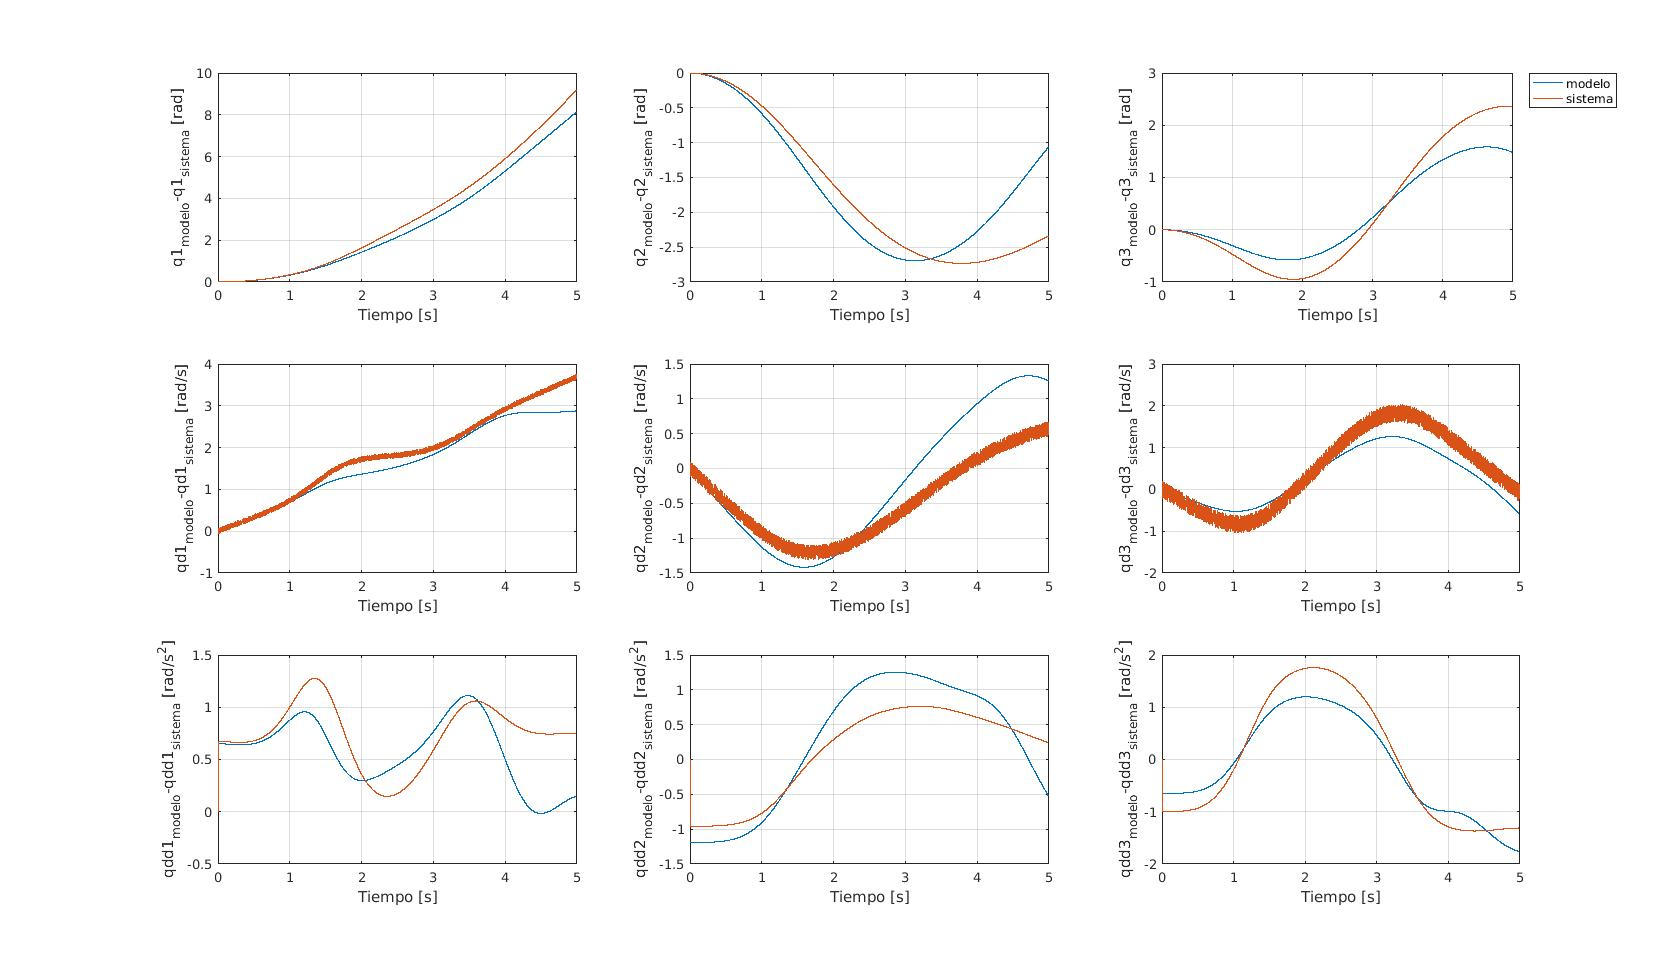
\includegraphics[width=1\textwidth]{EstimacParam_SisMod_In1_RealCR}
	\caption{Comparativa Variables articulares del modelo obtenido con medidas reales y reductoras}
\end{figure}

En éste caso, se observa cómo al emplear medidas reales para obtener el modelo dinámico del robot y al haber tenido que emplear filtros computacionales para conocer velocidades y aceleraciones del robot, el modelo obtenido no será tan bueno cómo en el caso en el que se usaron medidas ideales. Sin embargo, debido a que no posee un elevado orden de magnitud, se asumirá dicho error y se tomará el modelo cómo válido.\\
Ademas de ello, se observa que aparece cierto desfase entre el modelo obtenido y el robot real, éste desfase es debido a la aplicación de filtros a la señal. Cuando se emplean filtros hay que tener en cuenta que éstos introducen un cierto desfase, por tanto, será necesario encontrar un compomiso entre cuán bueno se quiere que sea el filtro y cuánto desfase se está dispuesto a asumir. En éste caso, debido a que nos encontramos en un proyecto basado en la simulación, se aceptará un cierto desfase a cambio de haber diseñado buenos filtros para las señales.

\newpage
Por tanto, la magnitud de los errores obtenidos se muestra a continuación:

\begin{figure}[h!]
	\centering
	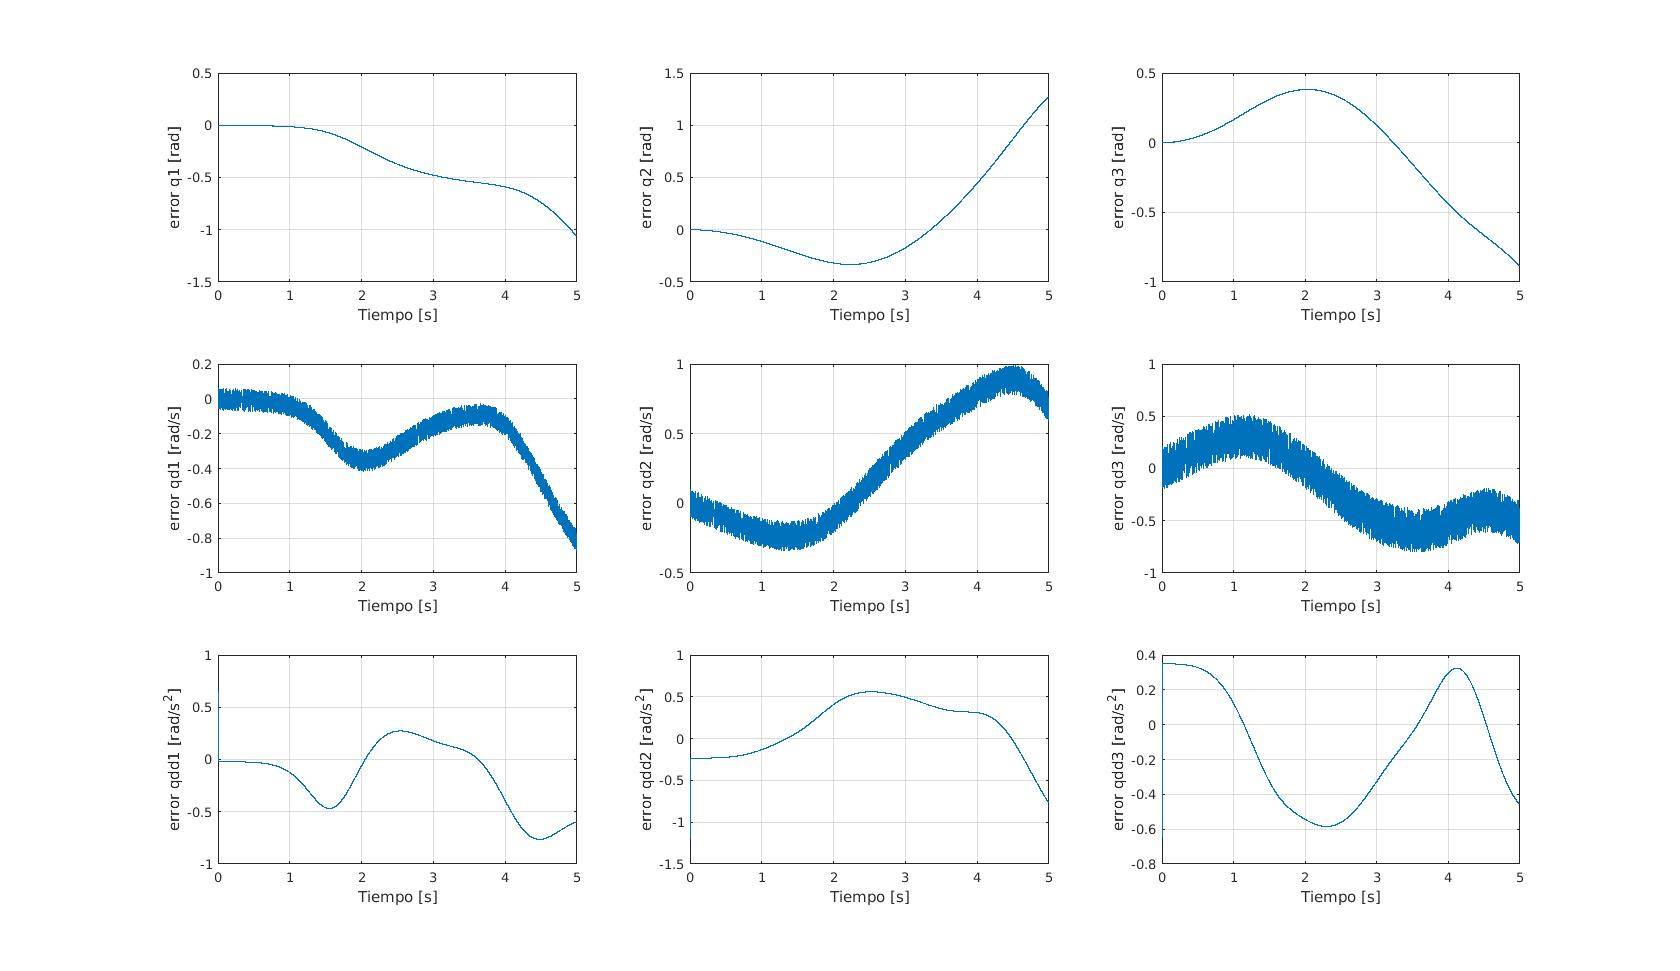
\includegraphics[width=1\textwidth]{EstimacParam_SisModError_In1_RealCR}
	\caption{Error del modelo obtenido con medidas reales y reductoras}
\end{figure}

\subsubsection{Robot medidas reales sin reductoras}

\newpage
\section{Control Dinámico del brazo}
En esta última parte del proyecto, una vez se conoce el modelo del robot en las diferentes configuraciones, se pasará a buscar implementar un control dinámico sobre el mismo.Para poder implementar controladores sobre nuestro robot, será necesario obtener una función de transferencia matemática a modo de modelo que se asemeje al robot real.\\
Una vez se tenga un modelo lineal de cada articulación del robot, junto con el generador de trayectorias creado anteriormente, se buscará que el robot siga una trayectoria predefinida. Básicamente, se busca que el robot se desplace de un punto a otro minimizando el error y del modo y a la velocidad que el usuario desee.\\

	\subsection{Obtención del modelo lineal de las articulaciones del brazo}
Para obtener la función de transferencia de cada articulación del robot, se linealizará la ecuación dinamica que define cada motor en un punto de equilibrio en torno a velocidades nulas. Por lo tanto, las consideraciones que se tendrán en cuenta para linealizar la ecuación dinamica que define el comportamiento de cada articulacion del robot son:
\begin{itemize}
	\item Velocidades de equilibrio
	\begin{center}
		$ \dot{q_{eq}}=0 rad/s $\\
		$ \dot{q} =\dot{q_{eq}}+\Delta\dot{q}$
	\end{center}
	\item Aceleraciones de equilibrio
\begin{center}
	$ \ddot{q_{eq}}=0 rad/s $\\
	$  $
	$ \ddot{q} =\ddot{q_{eq}}+\Delta\ddot{q}$
\end{center}
\end{itemize}

Ademas de ello, se aplicarán una serie de simplificaciones a la ecuación dinámica. A continuación, se mostrarán las ecuaciones dinámicas de los motores:\\
\begin{center}
	$$
	\begin{pmatrix}
	 \tau_{1} \\
	 \tau_{2} \\
	 \tau_ {3}
	\end{pmatrix}=
	\begin{pmatrix}
	Kt_{1}R_{1}Im_{1}  \\
	Kt_{2}R_{2}Im_{2}  \\
	Kt_{3}R_{3}Im_{3}
	\end{pmatrix} =
	\begin{pmatrix}
	Ma_{11} & Ma_{12} & Ma_{13}  \\
	Ma_{21} & Ma_{22} & Ma_{23}  \\
	Ma_{31} & Ma_{32} & Ma_{33}
	\end{pmatrix}
	\ddot{q}+
	\begin{pmatrix}
	Va_{1} \\
	Va_{2} \\
	Va_{3} \\
	\end{pmatrix}
	\dot{q}+
	\begin{pmatrix}
	Ga_{1}  \\
	Ga_{2}  \\
	Ga_{3}\\
	\end{pmatrix}
	$$
\end{center}
donde se asume que dentro de los términos de inercia y de Coirolis se han tenido en cuenta las inercias y fricciones viscosas de los motores.\\

La primera simplificación del modelo que se hará para poder linealizar el modelo en torno a un punto de operación, será suponer la matriz de inercias diagonal y, además de ello, se cogerá el valor medio de todos los senos y cosenos de tal modo que únicamente se tomen los valores de inercias medios. De manera praćtica, se harán cero todas las variables articulares del modelo. De éste modo, se desacoplará el sistema.\\
En cuando a la matriz de términos de Coirolis, únicamente aportarán a la linealización la fricción viscosa de los motores, es decir, se despreciarán todos los terminos exceptuando el que acompañe al valor de la velocidad articular.\\
Por último, la gravedad se despreciará para obtener un modelo, de tal modo que, se emplearán las siguientes ecuaciones para obtener los modelos de las articulaciones del robot:
\begin{equation}
	\begin{pmatrix}
	Kt_{1}R_{1}Im_{1}  \\
	Kt_{2}R_{2}Im_{2}  \\
	Kt_{3}R_{3}Im_{3}
	\end{pmatrix} =
	\begin{pmatrix}
	Ma_{11} & 0 	  & 0  \\
		0   & Ma_{22} & 0  \\
		0   & 0   	  & Ma_{33}
	\end{pmatrix}
	\ddot{q}+
	\begin{pmatrix}
	Va_{1} \\
	Va_{2} \\
	Va_{3} \\
	\end{pmatrix}
	\dot{q}
\end{equation}

A continuación, se obtendrá el modelo de la primera articulación y, el procedimiento será análogo para las restantes:
\begin{center}
	$Kt_{1}R_{1}Im_{1}(t)=Ma_{11}\ddot{q_{1}(t)} + Va_{1}\dot{q_{1}(t)}$
\end{center}
Se realizará una transformación al dominio de Laplace y, posteriormente, se expresará en forma de función de transferencia:
\begin{equation}
	Kt_{1}R_{1}Im_{1}(s)=s^{2}Ma_{11}q_{1}(s) + sVa_{1}q_{1}(s) \rightarrow \frac{q_{1}(s)}{Im_{1}(s)}=\frac{Kt_{1}R_{1}}{s(Ma_{11}s+Va_{1})}
\end{equation}

Por lo tanto, se definirá el modelo de cada articulación cómo:
\begin{equation}
	G_{1}(s)=\frac{Kt_{1}R_{1}}{s(Ma_{11}s+Va_{1})} \hspace{1cm} G_{2}(s)=\frac{Kt_{2}R_{2}}{s(Ma_{2}s+Va_{2})} \hspace{1cm} G_{3}(s)=\frac{Kt_{3}R_{3}}{s(Ma_{33}s+Va_{3})}
\end{equation}

	\subsection{Diseño de controladores}
	En éste apartado, se analizará cómo se hayarán los controladores que, posteriormente se implementarán sobre el robot para hacer que se desplace a lo largo de una trayectoria que se generará mediante el control cinemático.\\
	Cabe destacar que, en los controladores que se implementen junto con el compensador de gravedad, el de dinámica o el par calculado, la realimentación podrá ser por referencia, en lugar de emplear las medidas reales, de tal modo que se realimente con una señal sin ruido ni errores.\\
	\subsubsection{Controlador PD/PID}
	Para diseñar éstos controladores lineales, se empleará el modelo anteriormente mostrado y se implementarán directamente. El esquema de control será el esquema clásico de control, ya que éste tipo de controladores serán lo primeros en implementar y, por extensión, los más sencillos. \\
	La función de transferencia de los controladores a implementar será:\\
	\begin{equation}
		C(s)=K_{P}(T_{D}s+1) \hspace{2cm} C(s)=K_{P}\frac{T_{D}T_{I}s^{2}+T_{I}s+1}{T_{I}s}
	\end{equation}

	\subsubsection{Controlador PD/PID con compensación de gravedad}
	Para implementar éste controlador, se parte de la base de que, aunque la gravedad es una perturbación mantenida, se puede
modelar, ya que se conoce de la obtención del modelo dinámico los efectos de la gravedad en el modelo del robot.\\
Por tanto, para implementar un controlador con compensación de gravedad se le sumará a la señal de control generada por el
controlador diseñado anteriormente, los efectos de la gravedad en el robot.\\
Este bloque que añade los efectos de la gravedad tendrá como entrada la posición actual del robot (podría tener la referencia de posición) y la salida será la compensación de la señal de control. El esquema de montaje de éste tipo de control se muestra a continuación:

\begin{figure}[h!]
	\centering
	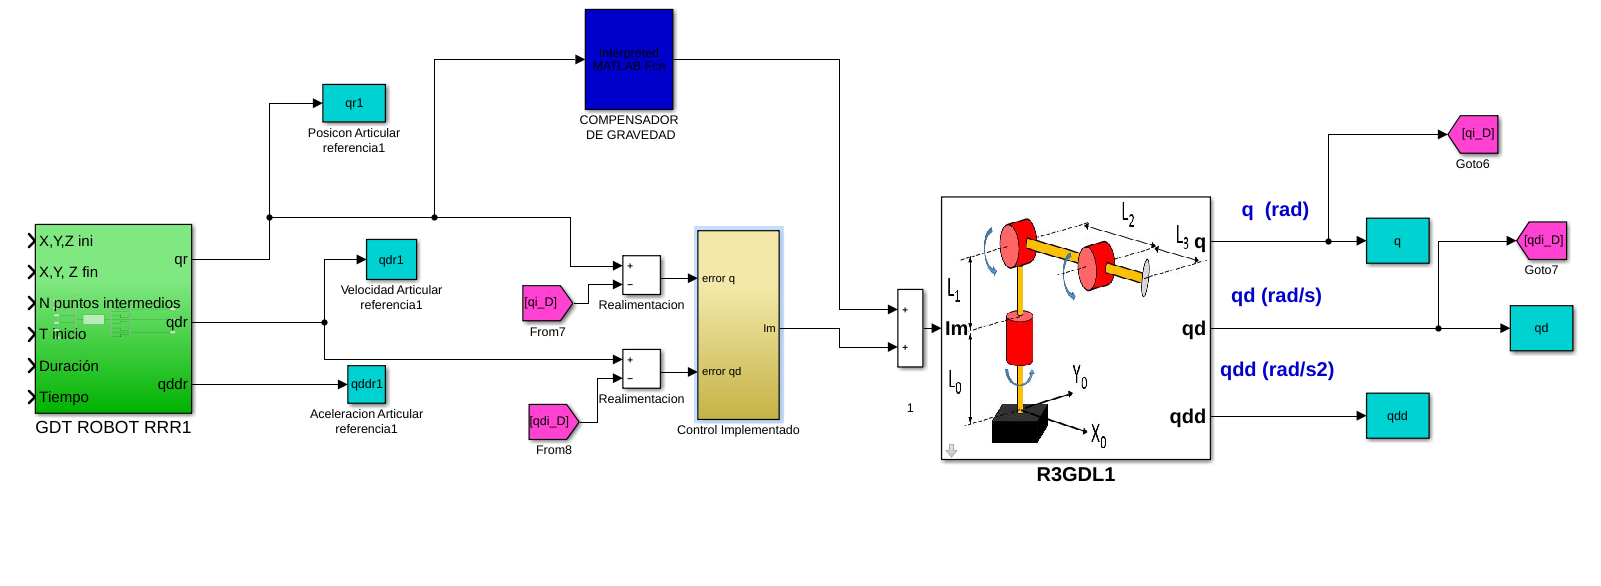
\includegraphics[width=.8\textwidth]{montaje_grav}
	\caption{Diagrama de control del compensador de gravedad}
\end{figure}

	\subsubsection{Controlador PD/PID con compensación de dinámica (Feedforward)}
	La implementación de controladores por precompensación de dinámica será la primera vez que se implementen controladores basados en modelo. La principal diferencia de éste tipo de controladores es que dependen en gran parte de la bondad del modelo obtenido, ya que se realimentará con el modelo dinámico inverso obtenido. Sin embargo, cabe destacar que en control de brazos manipuladores se emplea bastante debido a que se suele lograr obtener buenos modelos dinámicos de los robots.\\

	Para implementar éste controlador, también conocido como \textit{Feedforward}, se modificará el modelo de control de tal modo que se precompensen los efectos del modelo dinámico completo del robot, no solo la gravedad.
	\begin{equation}
		I_m= M_{A}(q)\ddot{q_{ref}} + C(q,\dot{q})\dot{q} + G_{A}(q) + u
	\end{equation}
cómo se observa, la señal de control generada estará formada por el modelo dinámico del robot más una señal adiccional,u.\\
Para conocer el valor de esa señal de control adiccional, se restará al modelo del sistema la señal de control que se desea generar de tal modo que se obtenga la expresión del bucle cerrado interno de control.
\begin{equation}
	\begin{array}{llll}
	  & Im=M_{A}(q)\ddot{q} + C_{A}(q,\dot{q})\dot{q} + G_{A}(q) \\
	- & Im=M_{A}(q)\ddot{q_{ref}} + C_{A}(q,\dot{q})\dot{q} + G_{A}(q) + u \\
	\cline{1-4}
	  & M_{A}(q)\tilde{\ddot{q}} = u & &
	\end{array}
\end{equation}
de ese modo se ha obtenido la señal de control adiccional, también conocida cómo la dinámica del error. Aunque no se lea correctamente, la ecuación obtenida es: $M_{A}(q)\tilde{\ddot{q}} = u$, dónde $\tilde{\ddot{q}}$ será el error en aceleración. \\
Habrá que diseñar controladores para la función de transferencia que se obtendrá a continuación. Para obtener dicha función de transferencia será necesario partir de condiciones iniciales nulas y transformarla al dominio de \textit{Laplace}.
\begin{equation}
	M_{A}(q)\tilde{\ddot{q}}(t) = u(t) \rightarrow M_{A}(q)\tilde{q}(s)s^{2} = u(s) \rightarrow \frac{\tilde{q}(s)}{u(s)}=\frac{K_{t}R}{M_{A}s^{2}}[\frac{ud.error}{ud.sc}]
\end{equation}

Se deberán diseñar tres funciones de transferencia, una por articulación. El esquema en diagrama de bloques de éste controlador se muestra a continuación:

\begin{figure}[h!]
	\centering
	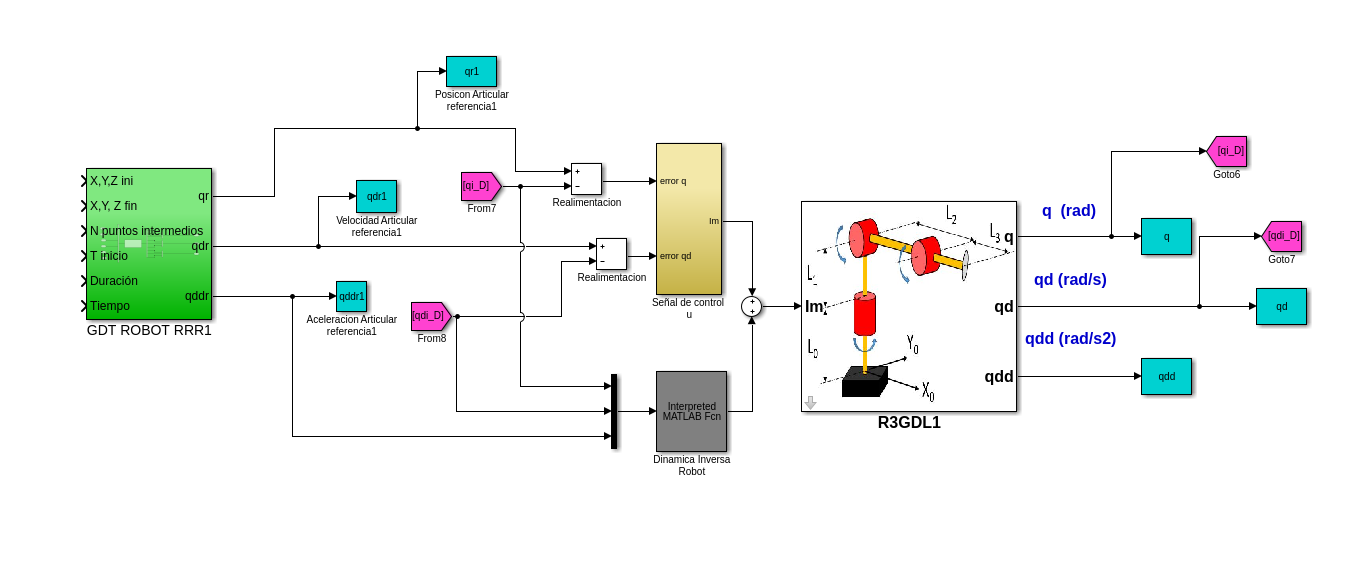
\includegraphics[width=.8\textwidth]{montaje_feedforward}
	\caption{Esquema de un controlador Feed Forward}
\end{figure}

debido a que no se puede medir la aceleración de las variables articulares, cómo se observa, el modelo dinámico inverso del robot se alimentará con los valores de las variables articulares en posición y velocidad y en el caso de la aceleración, se alimentará con la referencia obtenida del generador de trayectorias.

Por lo tanto, a modo de resumen, las funciones de transferencia de las cuales hará que obtener controladores son:
\begin{equation}
	G_{1}(s)=\frac{K_{t1}R_1}{M_{a11}s^{2}} \hspace{2cm} G_{2}(s)=\frac{K_{t2}R_2}{M_{a22}s^{2}} \hspace{2cm} G_{3}(s)=\frac{K_{t3}R_3}{M_{a33}s^{2}}
\end{equation}


	\subsubsection{Controlador PD/PID con par calculado}
	El control mediante par calculado será el último en implementar en éste proyecto. El par calculado se basa en la busqueda de desacoplar totalmente las interaciones del robot, resultando la dinámica del error cómo un doble integrador, para el cuál habrá que diseñar controladores. \\
	Que las articulaciones de un robot estén desacopladas implica que un par en un determinado actuador únicamente afectará al movimiento de dicha articulación.\\
	Por tanto, la diferencia de éste controlador frente al resto es que es un controlador dinámico. Además, es un controlador totalmente basado en el modelo, lo que conlleva que si el modelo es malo el control también lo será.
	Si, al igual que antes, se resta al sistema la señal de control que se desea implementar, se obtendrá la dinámica del error:
	\begin{equation}
		\begin{array}{llll}
		  & Im=M_{A}(q)\ddot{q} + C_{A}(q,\dot{q})\dot{q} + G_{A}(q) \\
		- & Im=M_{A}(q)\ddot{q_{ref}+u} + C_{A}(q,\dot{q})\dot{q} + G_{A}(q) \\
		\cline{1-4}
		\vspace{0.2cm}
		  & \tilde{\ddot{q}} = u & &
		\end{array}
	\end{equation}

	Por tanto, transformando la dinámica del error al dominio de \textit{Laplace}, las funciones de transferencia a partir de las cuales hay que diseñar los controladores serán:
	\begin{equation}
		G_{1}(s)=\frac{1}{s^{2}} \hspace{2cm} G_{2}(s)=\frac{1}{s^{2}} \hspace{2cm} G_{3}(s)=\frac{1}{s^{2}}
	\end{equation}

	Y, el esquema de control del par calculado se muestra a continuación:

		\begin{figure}[h!]
			\centering
			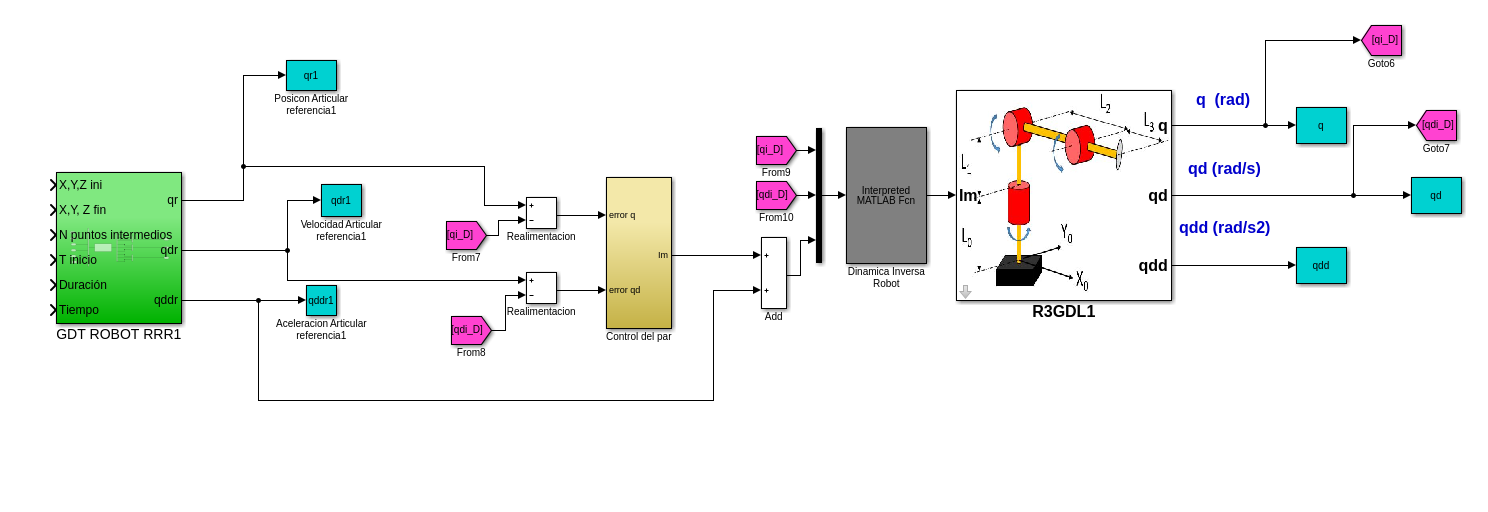
\includegraphics[width=.8\textwidth]{montaje_parcalcul}
			\caption{Esquema de un controlador Par Calculado}
		\end{figure}

\newpage
	\subsection{Analisis de experimentos para probar controladores}
En éste último apartado, se diseñarán diversos experimentos de control en los cuales se acentuen los efectos de un controlador u otro, por ejemplo, se realizarán trayectorias en las cuales se noten los efectos gravitatorios y así se observe la mejoría del controlador empleando un compensador de gravedad, etcétera.\\
Por tanto, los controladores que se van a implementar son los anteriores y los modelos a partir de los cuales se obtendrán serán el ideal y el real con y sin reductoras. También se diseñarán experimentos en el que se comparen los modelos obtenidos con medidas ideales y reales.\\

Por consiguiente, se realizarán los siguientes experimentos, en los cuales se definirá qué controladores se desea comparar y con qué fin:
\begin{itemize}
	\item En primer lugar, se realizará una comparativa entre los controladores PD y PID, de tal modo que se acentúe el efecto integral del PID y se observe la diferencia entre ambos controladores. Para ello, se generará una trayectoria relativamente lenta en la dirección negativa del eje Z, es decir, se partirá de la posición inicial del robot y se hará descender el brazo. \\

	\item Debido a que la principal perturbación que se tendrá es la gravedad, la cuál es una perturbación mantenida y conocida, la acometida del efecto integral será contrarestar ésta perturbación mantenida. Sin embargo, el principal problema del efecto integral es la agresividad del mismo. \\
	Por tanto, en éste caso, se comprobará si el error es menor al emplear un control PD con compensación de gravedad o un PID. En un ambiente real, teoricamente sería más correcto emplear el PD con la compensación para evitar los "latigazos" que podría llegar a generar en el robot el efecto integral.\\
	Seria conveniente para poder mostrar más correctamente éstos resultados buscar experimentos en los cuales se acentuen los efectos de la gravedad, para ello, lo ideal sería generar una trayectoria similar a la anterior pero en éste caso se emplearán los controladores diseñados para el robot real y se realimentarán con medidas reales. \\
	Es posible que, para mejorar el control, en lugar de realimentar el compensador de gravedad con la medida real de posición sea conveniente realimentarlo con la referencia de posición obtenida del generador de trayectorias. \\

	\item Posteriormente, se analizará el primer controlador basado en modelo, el control \textit{FeedForward}. En primer lugar sería convenientee realizar un análisis de cómo afecta la bondad del modelo a éste controlador comparando robot reales y robots ideales. \\
	Tras ello, se comprobará éste control realizando experimentos dónde se afectúen los términos de Coirolis, para ello sería conveniente realizar trayectorias ... .\\

	\item Finalmente, se analizará el controlador par calculado, el cuál se basará en desacoplar totalmente las articulaciones del robot, de tal modo que el modelo de cada articulación resulte en un doble integrador.\\
	Sería conveniente analizar trayectorias en las que se acentúen los términos inerciales del brazo robótico, ya que en éste caso se busca compensar todo el modelo.\\
	Teóricamente, si el modelo obtenido es buen modelo, debería ser el mejor controlador implementado.\\

	\item Además de todo, sería conveniente comparar el resultado del emplear una realimentación de los controladores con medidas reales o con referencia, ya que al realimentar con la referencia, se obtendrá una medida mucho más limpia y que, como es de esperar, generará un menor error. Este estudio sería conveniente en el caso de emplear los modelos con medidas reales obtenidos.\\
\end{itemize}

\newpage
\subsubsection{Comparativa controladores PD-PID ideales con reductoras}
En éste experimento, se compararán los controladores diseñados a partir del modelo ideal con reductoras. \\
La trayectoria que se empleará para éste experimentos se muestra a continuación gráficamente:
\begin{figure}[h!]
	\centering
	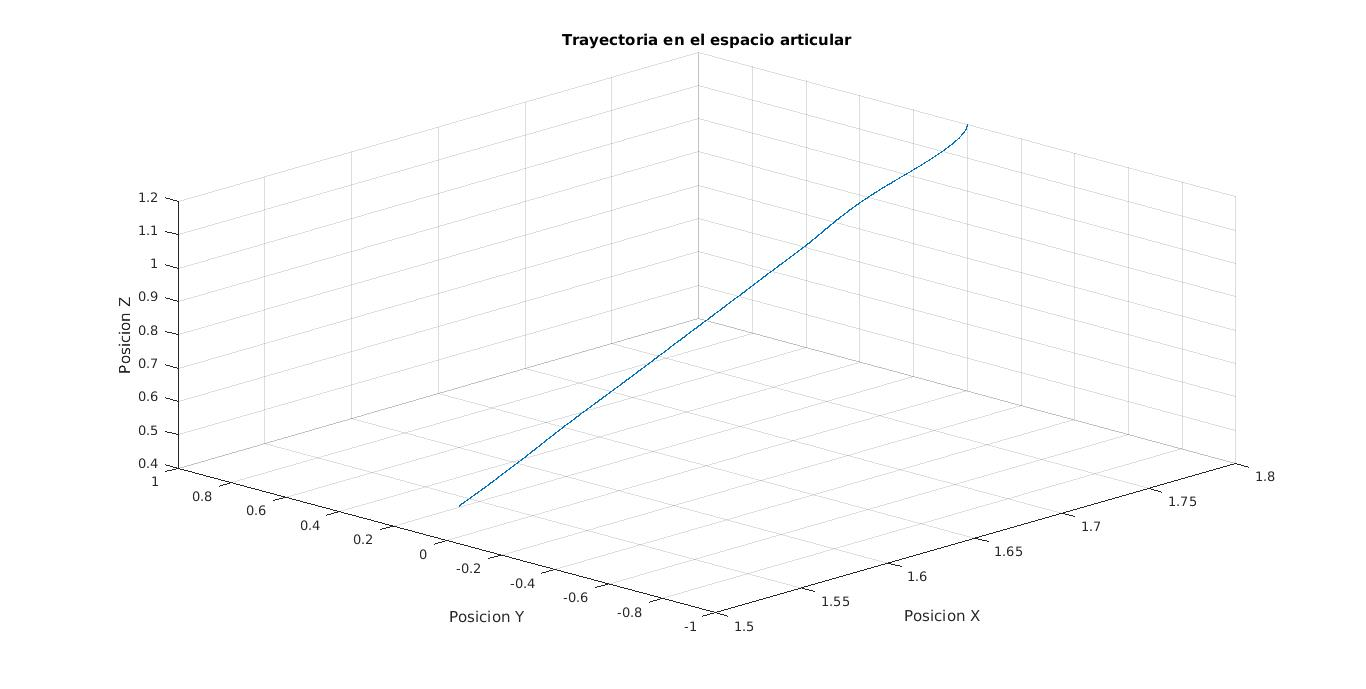
\includegraphics[width=.8\textwidth]{exp1_tray}
	\caption{Trayectoria diseñada para evaluar el efecto integral de los controladores}
\end{figure}

Cómo se ha dicho anteriormente, con éste experimento se busca evaluar el efecto integral del controlador, lo que conllevará que cuando se implemente el PID el error en regimen permamente tenderá a ser nulo, sin embargo en el caso del PD se tendrá un error mantenido.\\
Se comparará el error en posición de las tres articulaciones, ya que es dónde se observa dicho efecto:
\begin{itemize}
	\item \textbf{Controlador PD}

	\begin{figure}[h!]
		\centering
		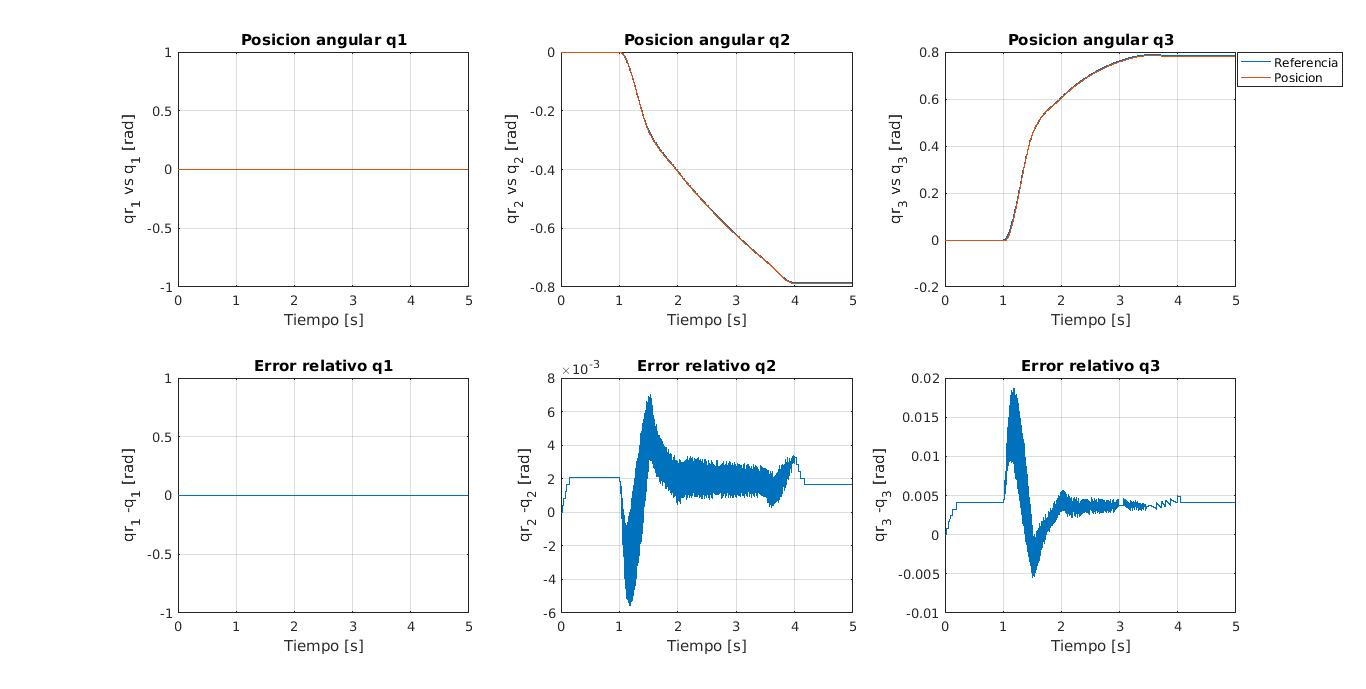
\includegraphics[width=.8\textwidth]{exp1_posPD}
		\caption{Seguimiento de referencia en posición con el controlador PD}
	\end{figure}

\newpage
	\item \textbf{Controlador PID}
	\begin{figure}[h!]
		\centering
		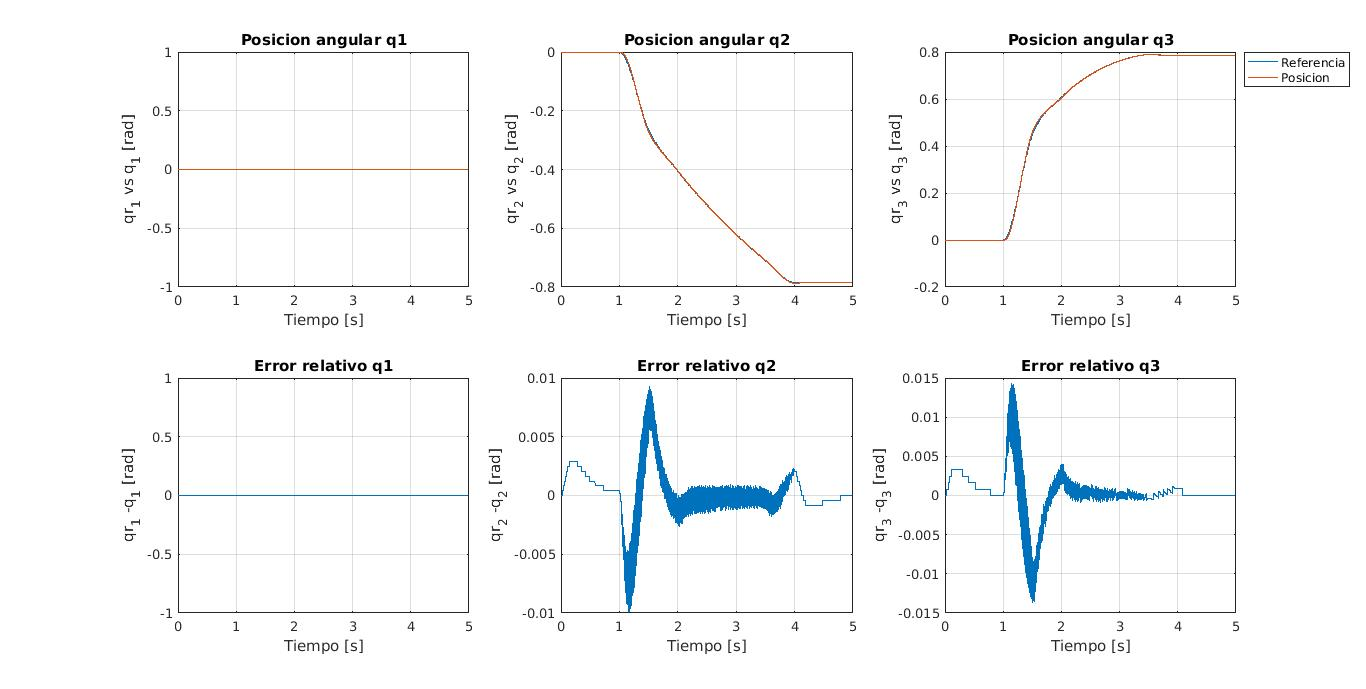
\includegraphics[width=.8\textwidth]{exp1_posPID}
		\caption{Seguimiento de referencia en posición con el controlador PID}
	\end{figure}

\end{itemize}

Se observa claramente cómo el efecto integral compensa la perturbación mantenida que es la gravedad, por tanto, el controlador PID mejora la respuesta del PD asumiento la agresividad del efecto integral.

\subsubsection{Comparativa controlador PID Y PD con compensacion gravedad}
En éste caso, se implementarán los controladores diseñados en base al modelo del robot real con reductoras. Debido a que se han empleado medidas reales, se realimentarán con las medidas reales del robot. Si la respuesta no fuese lo suficientemente aceptable, se alimentaría el compensador de gravedad con la referencia obtenida del generador de trayectorias. \\
Se ha optado por emplear la misma trayectoria que anteriormente debido a que se busca que se acentuen los efectos asociados a los terminos gravitatorios, al igual que antes.\\
Si se compara el resultado obtenido anteriormente con el PID a partir del modelo ideal con el resultado obtenido al implementar un controlador PD con compensador de gravedad, se observa que éste segundo nos dará unos mejores resultados en el seguimiento de la trayectoria y una menor magnitud del error. La grafica de seguimiento se muestra a continuación:

\begin{figure}[h!]
	\centering
	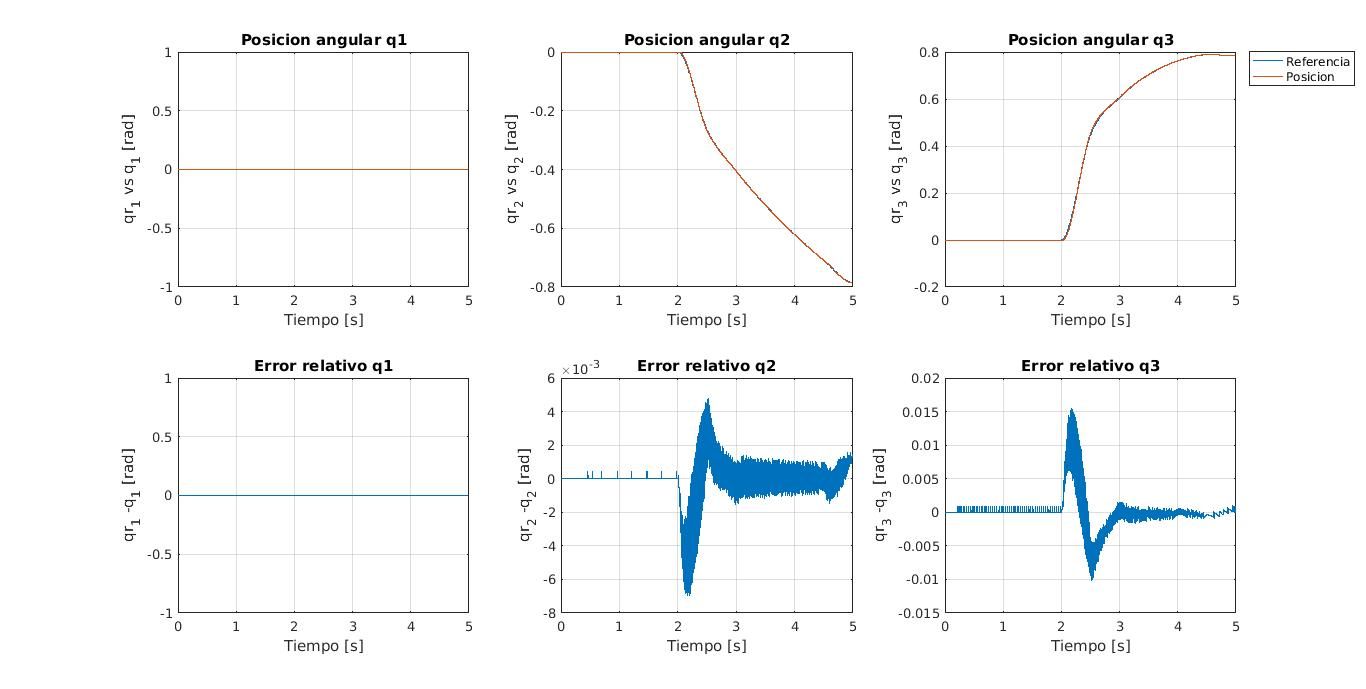
\includegraphics[width=.8\textwidth]{exp2_posPDcomp}
	\caption{Seguimiento de referencia en posición con el controlador PD con compensación de gravedad}
\end{figure}

%Si en lugar de realimentar el compensador con la medida real de posición, es decir, la que se obtiene de los encoders, se realimenta con %la referencia que dá el generador de trayectorias el resultado es notablemente mejor, ésto es debido a que se está realimentando con una %señal límpia.

\subsubsection{Comparativa del control con compensación de dinámica o \textit{FeedForward}}
En éste apartado, se comprobará la bondad de los modelos obtenidos. Para ello, implementará la primera técnica de control avanzado que se dispone, la cuál es el control con compensación de dinámica.\\
Por tanto, para éste controlador se diseñará un controlador PD o PID que compense la dinámica del error y se compensará la dinámica del robot, en concreto los términos de Coirolis.\\

Se deberá buscar un experimento en el cuál se acentúen los terminos de Coirolis, por ello se ha optado por emplear el que se muestra a continuación, el cuál es un movimientos que contiene giro sobre la base en un tiempo medio, es decir, ni excesivamente rápido ni lento. \\
La trayectoria que se empleará para éste experimento partirá de las variables articulares nulas y girará sobre sí mismo bajando el brazo, intentando acentuar los términos de Coirolis.\\

Inicialmente, se comparará la bondad de los modelos obtenidos con reductoras. Por tanto, a continuación se mostrará el seguimiento de la trayectoria en el plano XYZ y el seguimiento de la referencia en posición de las variables articulares, tras ello, se sacarán una serie de conclusiones:
\begin{itemize}
	\item \textbf{Robot ideal con reductoras}
	El seguimiento de la trayectoria en el plano XYZ será:
	\begin{figure}[h!]
		\centering
		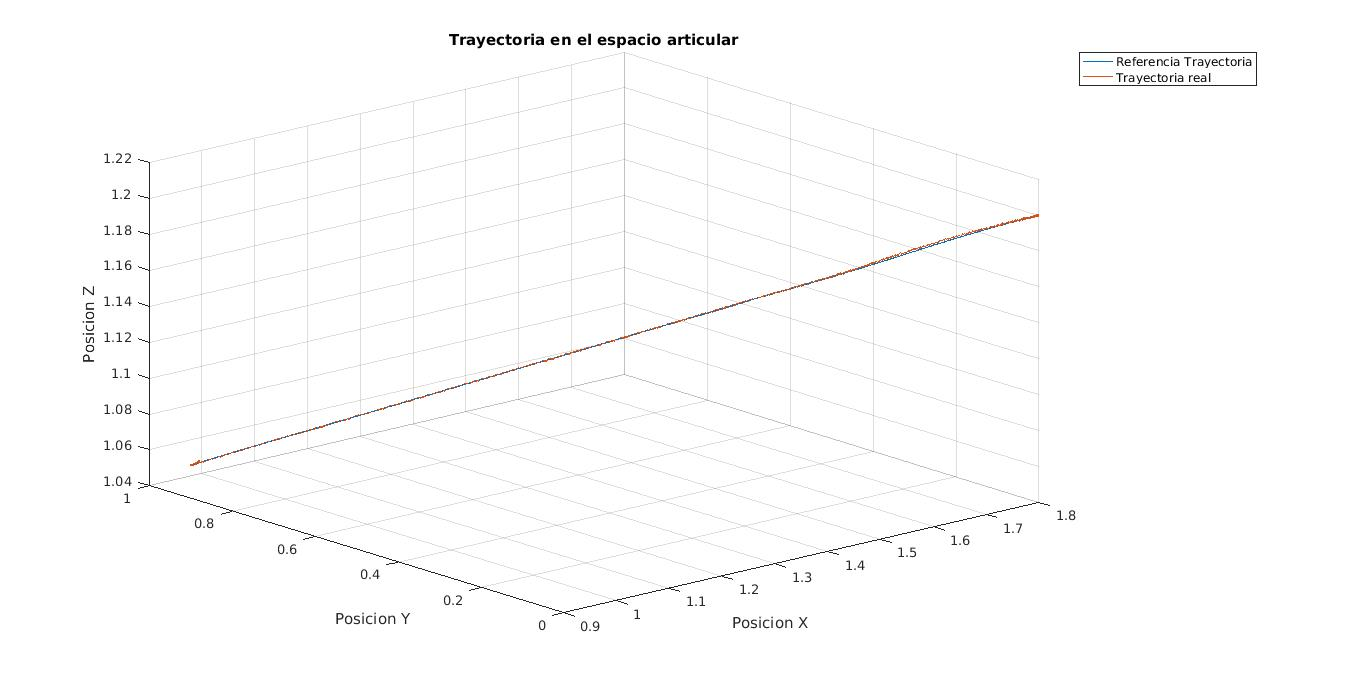
\includegraphics[width=.7\textwidth]{exp3_trayPDideal}
		\caption{Seguimiento de la trayectoria en el plano XYZ}
	\end{figure}

	Se observa cómo, a primera vista, se ha obtenido un buen modelo, ya que el seguimiento será bastante bueno. A continuación se verá cómo siguen la referencia de posición las variables articulares del robot:

	\begin{figure}[h!]
		\centering
		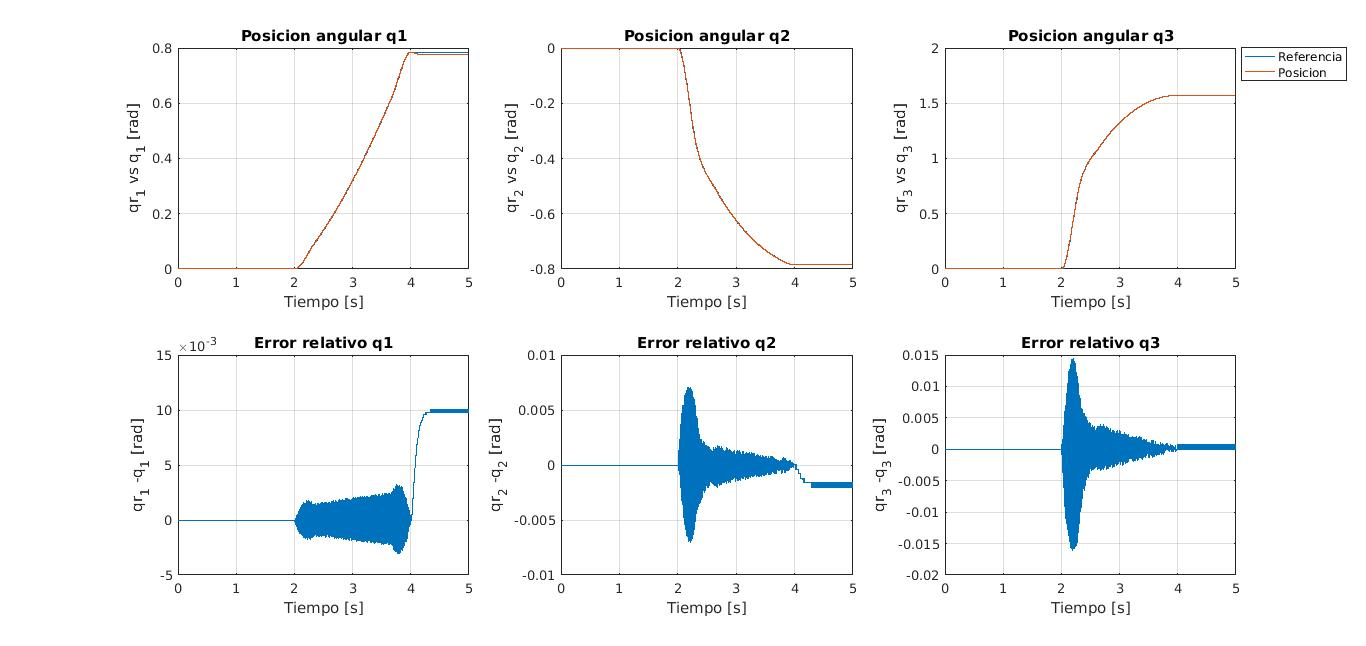
\includegraphics[width=.8\textwidth]{exp3_posPDidealCR}
		\caption{Seguimiento de referencia en posición de las variables articulares}
	\end{figure}

\newpage
	Aunque se aprecia un cierto error, la magnitud de éste es pequeña y, por tanto, fácilmente asumible. También cabe destacar que, la segunda articulación quizá se haya estimado algo peor, ya que es la que presenta error en regimen permanente tras la trayectoria. \\

	\item \textbf{Robot real con reductoras}
	El seguimiento de la trayectoria en el plano XYZ será:

	\begin{figure}[h!]
		\centering
		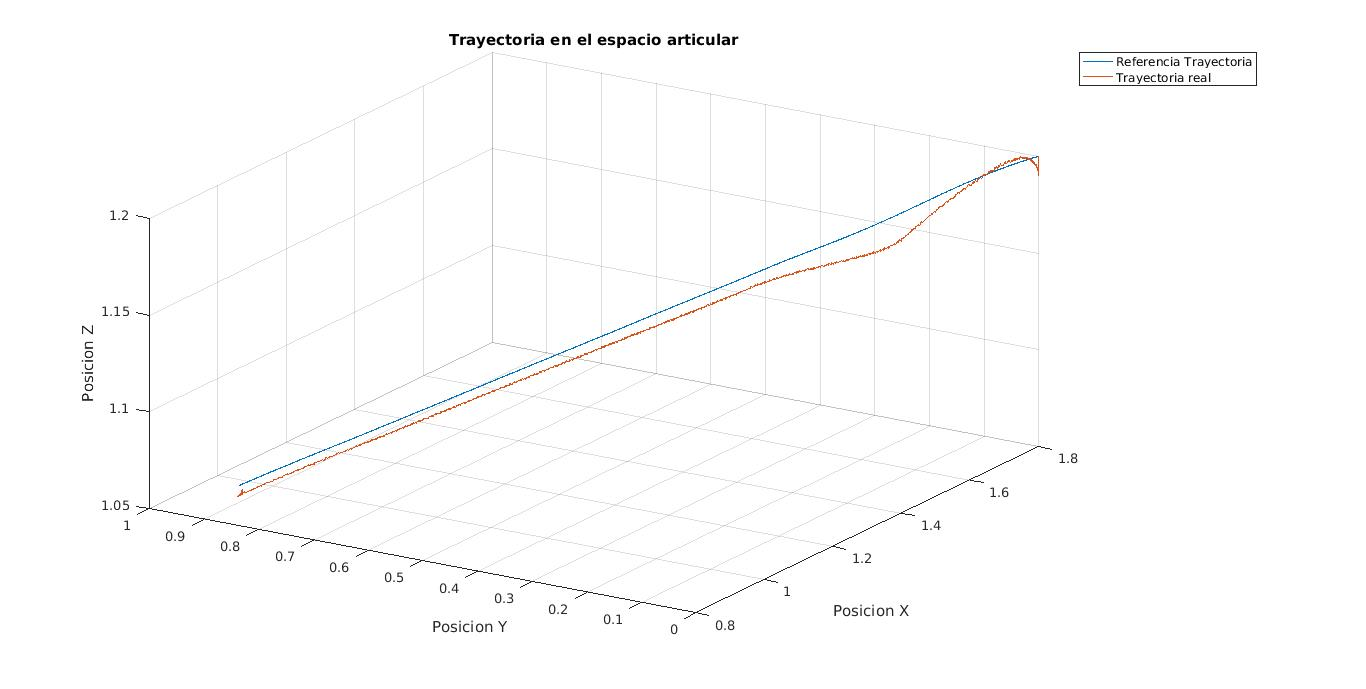
\includegraphics[width=.8\textwidth]{exp3_trayPDreal}
		\caption{Seguimiento de la trayectoria en el plano XYZ}
	\end{figure}

	En éste caso, debido a que se han tomado medidas reales para obtener el modelo del robot, se observa que se tendrá un error mantenido en el seguimiento de la trayectoria en el plano XYZ. Para analizar con mayor exactitud dicho error, es conveniente observar el seguimiento a referencia en posición realizado por las variables articuales del robot:

	\begin{figure}[h!]
		\centering
		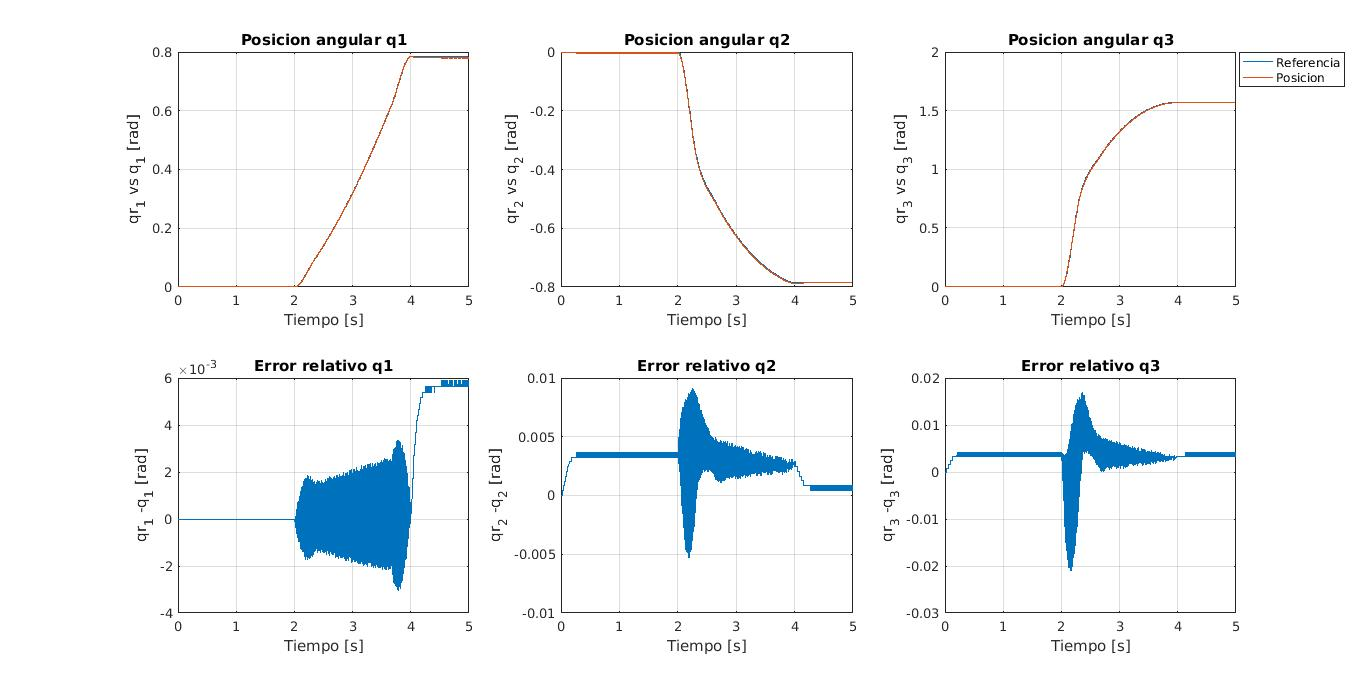
\includegraphics[width=.8\textwidth]{exp3_posPDrealCR}
		\caption{Seguimiento de referencia de las variables articulares}
	\end{figure}

Se puede observar que todas las variables articulares tras la trayectoría presentarán un error mantenido, sin embargo, la magnitud del mismo será pequeña.\\
Por tanto, se puede estimar que no se ha obtenido un mal modelo real del robot con reductoras, aunque no es perfecto, ni tan bueno cómo el ideal, será un modelo válido para trabajar con el mismo.

\end{itemize}

\newpage
\subsubsection{Comparativa del control par calculado}
En el controlador mediante par calculado se ha desacoplado totalmente las articulaciones del robot, de tal modo que la dinámica del error resultante es un doble integrador. \\
Además de ello, se notará más éste controlador cuando se trabaje sin reductoras, ya que las reductoras son las encargadas de desacoplar las articulaciones del robot, por tanto, si no se emplean reductoras, el encargado de desacoplar las articulaciones será el propio control implementado. \\
Además de ello, también se buscará mostrar que, cuán más rápido se busque que sea el control, mayores serán los errores que se tendrán.\\

Por tanto, en primer lugar se empleará el robot ideal sin reductoras para mostrar el efecto de pedir mayor velocidad en el movimiento del robot y, posteriormente, se comparará el modelo ideal sin reductoras y el modelo real sin reductoras.\\
La trayectoria elegida será una trayectoria ascendente y de rotación que partirá de la posición inicial del robot.

\begin{itemize}
	\item \textbf{Comprobación del efecto del aumento de la velocidad en la trayectoria}
	A continuación, en primer lugar se mostrará la comparativa del seguimiento de la trayectoria en el espacio articular XYZ en función del la velocidad pedida para que siga la misma. Además, cabe destacar que se ha implementado un control PD para la dinámica del error.\\
	En primer lugar se mostrará la gráfica en la que se pedía que recorriese la trayectoria en 2 segundos, es decir, la que sería la trayectoria lenta:

	\begin{figure}[h!]
		\centering
		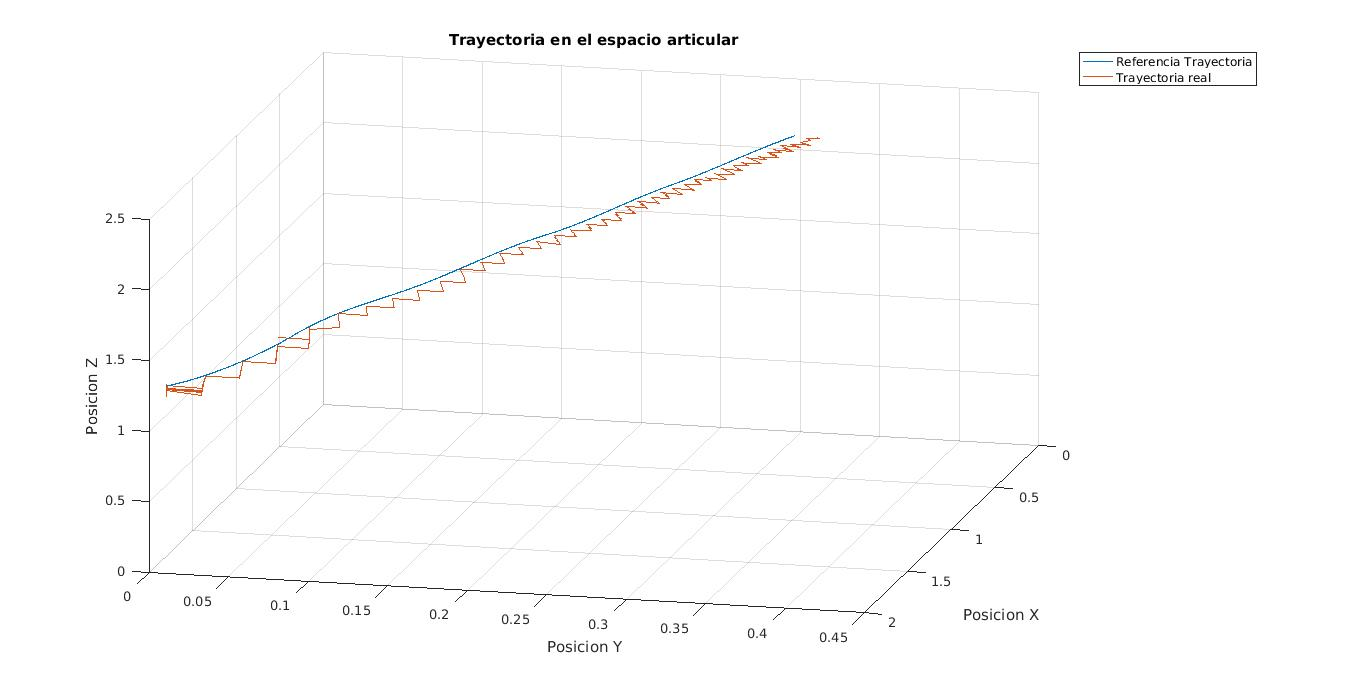
\includegraphics[width=.8\textwidth]{exp4_trayPDidealSR_lento}
		\caption{Seguimiento de la trayectoria lenta en el plano XYZ}
	\end{figure}

	Ahora, se mostrará el seguimiento en posiciones articulares cuando se pide que se siga la trayectoria algo más lenta:

	\begin{figure}[h!]
		\centering
		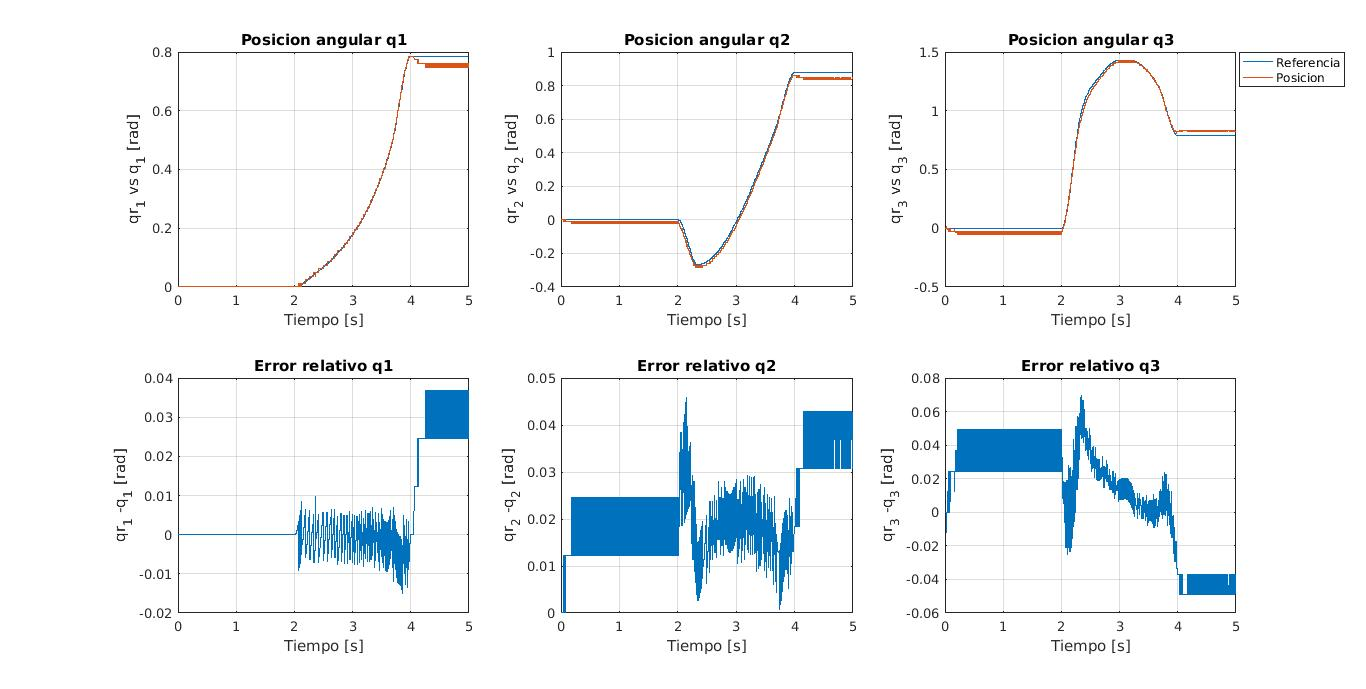
\includegraphics[width=.8\textwidth]{exp4_posPDidealSR_lento}
		\caption{Seguimiento de las variables articulares}
	\end{figure}

\newpage
Se observa que, aunque existe un error en las tres variables, éste error es significativamente pequeño y asumible en el control del robot.\\
Sin embargo, en el caso de que se pida que realice la trayectoria en la mitad de tiempo, el error se incrementará significativamente cómo se muestra a continuación:

\begin{figure}[h!]
	\centering
	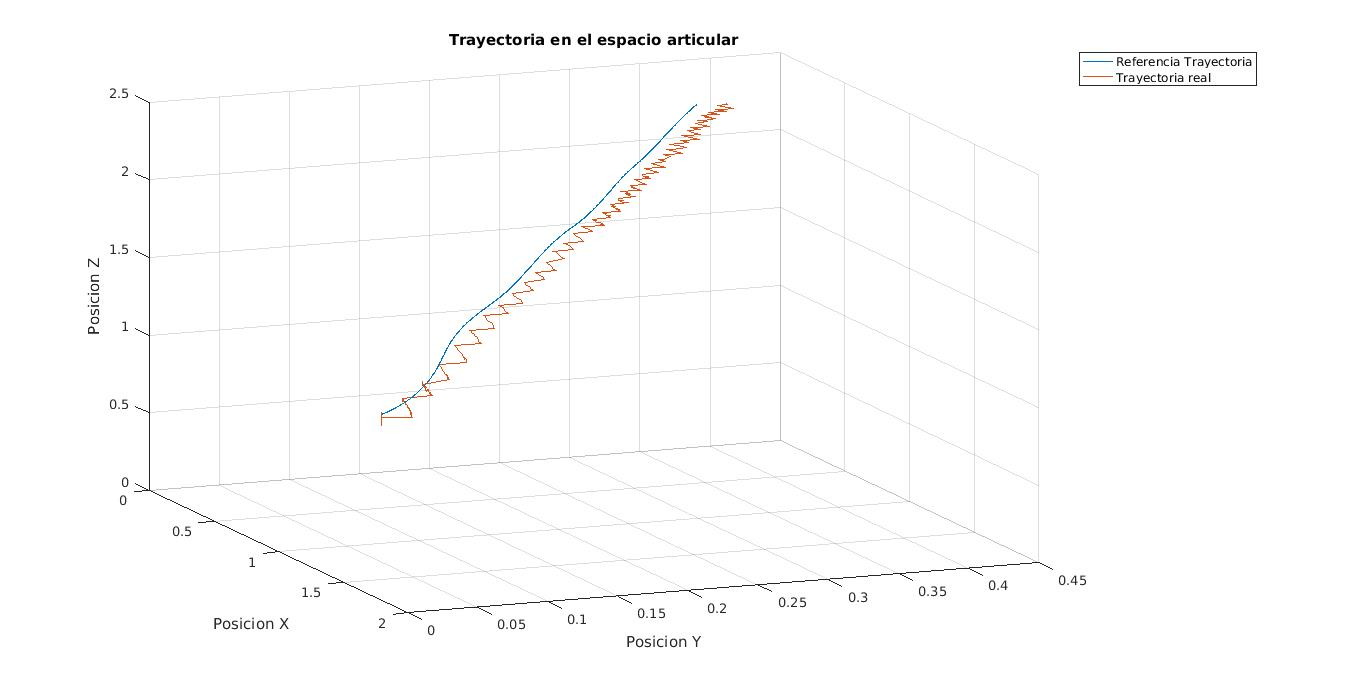
\includegraphics[width=.8\textwidth]{exp4_trayPDidealSR_rapido}
	\caption{Seguimiento de la trayectoria rapida en el plano XYZ}
\end{figure}

\newpage
Ahora, se mostrará el seguimiento en posiciones articulares cuando se pide que se siga la trayectoria en el doble de tiempo:

\begin{figure}[h!]
	\centering
	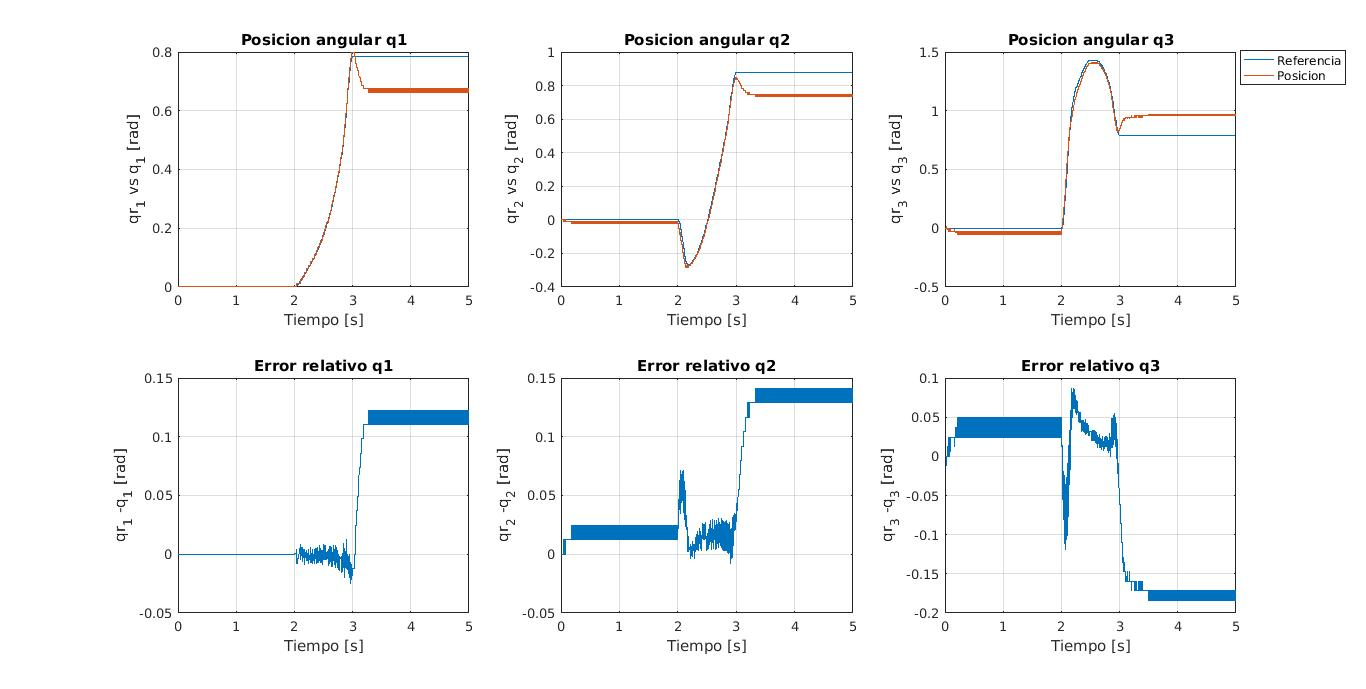
\includegraphics[width=.8\textwidth]{exp4_posPDidealSR_rapido}
	\caption{Seguimiento de las variables articulares}
\end{figure}

Por tanto, a modo de conclusión cabe destacar que, en el momento de pedirle al robot que siga una trayectoría será necesario hayar un compromiso entre la velocidad de la trayectoria y el error que se esté dispuesto a asumir en la misma.\\

	\item \textbf{Comparativa del modelo ideal sin reductoras obtenido y el real}

HAY QUE DEFINIR BIEN EL ROBOT REAL SIN REDUCTORAS PARA TERMINAR ÉSTE APARTADO. \\

\end{itemize}

\newpage
\section{Anexos}
	\subsection{Conclusiones (A LO MEJON SI A LO MEJON NO)}
	\subsection{Codigos de programacion}
	\subsection{Montajes en Simulink}

\end{document}
